\documentclass[12pt]{article}

% Packages
\usepackage{amsmath, amsthm, amssymb, mathrsfs}
\usepackage{mathtools}
\usepackage{relsize}
\usepackage{tikz}
\usetikzlibrary{arrows.meta}
\usepackage{hyperref}
\usepackage{geometry}
\geometry{a4paper, margin=1in}

% Environments
\newtheorem{theorem}{Theorem}
\newtheorem{lemma}{Lemma}
\newtheorem{definition}{Definition}
\newtheorem{problem}{Problem}
\newtheorem{exercise}{Exercise}
\newcommand{\defeq}{\stackrel{\mathclap{\mathsmaller{\text{def}}}}{=}}

\begin{document}
	% Title
	\title{My Notes for Discrete Probability: Detailed Explanations on Concepts and Proofs}
	\author{Mohamed Syaheer Altaf}
	\maketitle
	
	% Part 1: Events and Probability
	\section{Events and Probability}
	In this note, we consider only discrete probability spaces. Recall some basic terminologies:
	\begin{itemize}
		\item \textbf{Experiment:} any procedure whose outcomes are well-defined and which is repeatable indefinitely.
		\item \textbf{Sample space:} the set of all possible, well-defined outcomes of an experiment.
		\item \textbf{Event:} a subset of the sample space.
	\end{itemize}
	
	\subsection{Probability}
	\begin{definition}[Probability Space]
		A probability space has three components:\\
		\begin{enumerate}
			\item a sample space $\Omega$.
			\item a family of sets $\mathcal{F}$ representing \textbf{events}, where each set in $\mathcal{F}$ is a subset of the sample space $\Omega$ (i.e., $\mathcal{F} = 2^{\Omega}$).
			\item a probability function $\text{Pr}:\mathcal{F} \longrightarrow \mathbb{R}$ satisfying Definition~\ref{axioms}.
		\end{enumerate}
		\label{probability_space}
	\end{definition}
	
	\begin{definition}[Probability Axioms]
		A probability function is any function $\text{Pr}:\mathcal{F} \longrightarrow \mathbb{R}$ that satisfies the following conditions:\\
		\begin{enumerate}
			\item For any event $\mathcal{E} \in \mathcal{F}$, $\text{Pr}(\mathcal{E}) \geq 0$.
			\item $\text{Pr}(\Omega) = 1$.
			\item For any finite or countably infinite sequence of \textbf{pairwise mutually disjoint} events $\mathcal{E}_1,\mathcal{E}_2,\mathcal{E}_3,\dots,$\\
			$$\text{Pr}\Bigl(\bigcup_{i \geq 1}\mathcal{E}_i\Bigr) = \sum_{i \geq 1}\text{Pr}(\mathcal{E}_i)\text{.}$$
		\end{enumerate}
		\label{axioms}
	\end{definition}
	
	\begin{lemma}[Inclusion-Exclusion Principle]
		Let $\mathcal{E}_1,\mathcal{E}_2,\dots,\mathcal{E}_n$ be any $n$ events. Then
		$$\text{Pr}\Bigl(\bigcup_{i=1}^{n}\mathcal{E}_i\Bigr)=\sum_{i=1}^{n}\text{Pr}(\mathcal{E}_i)-\sum_{1 \leq i<j \leq n}\text{Pr}(\mathcal{E}_i \cap \mathcal{E}_j)+\sum_{1 \leq i<j<k \leq n}\text{Pr}(\mathcal{E}_i \cap \mathcal{E}_j \cap \mathcal{E}_k)- \dots + (-1)^{n+1}\text{Pr}\Bigl(\bigcap_{i=1}^{n}\mathcal{E}_i\Bigr)\text{.}$$
		\label{pie}
	\end{lemma}
	\begin{proof}
		We prove the \textbf{inclusion-exclusion principle} using mathematical induction. 
		
		\textbf{Base Case:} For $n=2$, consider two events $\mathcal{E}_1$ and $\mathcal{E}_2$. Note that:
		\begin{enumerate}
			\item $\text{Pr}(\mathcal{E}_1) = \text{Pr}\Bigl(\mathcal{E}_1 \setminus (\mathcal{E}_1 \cap \mathcal{E}_2)\Bigr) + \text{Pr}(\mathcal{E}_1 \cap \mathcal{E}_2)$, and
			\item $\text{Pr}(\mathcal{E}_2) = \text{Pr}\Bigl(\mathcal{E}_2 \setminus (\mathcal{E}_1 \cap \mathcal{E}_2)\Bigr) + \text{Pr}(\mathcal{E}_1 \cap \mathcal{E}_2)$.
		\end{enumerate}
		Thus,
		\begin{align*}
			\text{Pr}(\mathcal{E}_1 \cup \mathcal{E}_2) 
			&= \text{Pr}\Bigl(\mathcal{E}_1 \setminus (\mathcal{E}_1 \cap \mathcal{E}_2)\Bigr)
			+ \text{Pr}\Bigl(\mathcal{E}_2 \setminus (\mathcal{E}_1 \cap \mathcal{E}_2)\Bigr)
			+ \text{Pr}(\mathcal{E}_1 \cap \mathcal{E}_2)\\[.5em]
			&= \Bigl(\text{Pr}(\mathcal{E}_1) - \text{Pr}(\mathcal{E}_1 \cap \mathcal{E}_2)\Bigr)
			+ \Bigl(\text{Pr}(\mathcal{E}_2) - \text{Pr}(\mathcal{E}_1 \cap \mathcal{E}_2)\Bigr)
			+ \text{Pr}(\mathcal{E}_1 \cap \mathcal{E}_2)\\[.5em]
			&= \text{Pr}(\mathcal{E}_1) + \text{Pr}(\mathcal{E}_2) - \text{Pr}(\mathcal{E}_1 \cap \mathcal{E}_2)\text{.}
		\end{align*}
		This concludes the proof for the base case.
		
		\textbf{Induction Step:} Assume the identity holds for all $n=k$. We wish to show it holds for $n=k+1$. Consider
		\[
		\text{Pr}\Bigl(\bigcup_{i=1}^{k+1}\mathcal{E}_i\Bigr)
		= \text{Pr}\Bigl(\Bigl(\bigcup_{i=1}^{k}\mathcal{E}_i\Bigr) \cup \mathcal{E}_{k+1}\Bigr)\, .
		\]
		By the base case, we have
		\begin{align*}
			\text{Pr}\Bigl(\Bigl(\bigcup_{i=1}^{k}\mathcal{E}_i\Bigr) \cup \mathcal{E}_{k+1}\Bigr)
			&= \text{Pr}\Bigl(\bigcup_{i=1}^{k}\mathcal{E}_i\Bigr) + \text{Pr}(\mathcal{E}_{k+1}) - \text{Pr}\Bigl(\Bigl(\bigcup_{i=1}^{k}\mathcal{E}_i\Bigr) \cap \mathcal{E}_{k+1}\Bigr)\\
			&= \text{Pr}\Bigl(\bigcup_{i=1}^{k}\mathcal{E}_i\Bigr) + \text{Pr}(\mathcal{E}_{k+1})
			- \text{Pr}\Bigl((\mathcal{E}_1 \cap \mathcal{E}_{k+1}) \cup \dots \cup (\mathcal{E}_k \cap \mathcal{E}_{k+1})\Bigr)\text{.}\\
		\end{align*}
		The final equality is due to the \textbf{distributive law} in set theory. Note that both $\text{Pr}\Bigl(\bigcup_{i=1}^{k}\mathcal{E}_i\Bigr)$ and $\text{Pr}\Bigl((\mathcal{E}_1 \cap \mathcal{E}_{k+1}) \cup \dots \cup (\mathcal{E}_k \cap \mathcal{E}_{k+1})\Bigr)$
		can be expressed using the induction hypothesis. Substituting these expressed terms back into the equation above completes the induction.
		
		For clarity, the expression for the last term is given by:
		\begin{align*}
			\text{Pr}\Bigl((\mathcal{E}_1 \cap \mathcal{E}_{k+1}) \cup \dots \cup (\mathcal{E}_k \cap \mathcal{E}_{k+1})\Bigr)
			&= \sum_{i=1}^{k}\text{Pr}(\mathcal{E}_i \cap \mathcal{E}_{k+1})
			- \sum_{1 \leq i<j \leq k}\text{Pr}(\mathcal{E}_i \cap \mathcal{E}_j \cap \mathcal{E}_{k+1})\\
			&\quad + \dots + (-1)^{k+1}\text{Pr}\Bigl(\bigcap_{i=1}^{k+1}\mathcal{E}_i\Bigr)\text{.}
		\end{align*}
		This completes the proof.
	\end{proof}
	
	\begin{definition}[Independence]
		Two events $\mathcal{E}_1$ and $\mathcal{E}_2$ are \textbf{independent} if and only if
		$$\text{Pr}(\mathcal{E}_1 \cap \mathcal{E}_2)=\text{Pr}(\mathcal{E}_1)\cdot \text{Pr}(\mathcal{E}_2)\text{.}$$\\
		More generally, events $\mathcal{E}_1,\mathcal{E}_2,\dots,\mathcal{E}_k$ are \textbf{mutually independent} if and only if, for any subset $I \subseteq \{1,2,\dots,k\}$,
		$$\text{Pr}\Bigl(\bigcap_{i \in I}\mathcal{E}_i\Bigr)=\prod_{i \in I}\text{Pr}(\mathcal{E}_i)\text{.}$$\\
		A simple computation shows that the number of unique, unordered subsets (i.e., the number of conditions required to establish mutual independence) for a collection of $n$ events is given by:
		$$\binom{n}{2}+\binom{n}{3}+\dots+\binom{n}{n-1}+\binom{n}{n}\text{.}$$
		\label{independence}
	\end{definition}
	
	For example, if we have a collection of three events $\mathcal{E}_1$, $\mathcal{E}_2$, and $\mathcal{E}_3$, independence amounts to satisfying these four conditions:\\
	$$\text{Pr}(\mathcal{E}_1 \cap \mathcal{E}_2)=\text{Pr}(\mathcal{E}_1)\cdot \text{Pr}(\mathcal{E}_2)\text{,}$$\\
	$$\text{Pr}(\mathcal{E}_1 \cap \mathcal{E}_3)=\text{Pr}(\mathcal{E}_1)\cdot \text{Pr}(\mathcal{E}_3)\text{,}$$\\
	$$\text{Pr}(\mathcal{E}_2 \cap \mathcal{E}_3)=\text{Pr}(\mathcal{E}_2)\cdot \text{Pr}(\mathcal{E}_3)\text{, and}$$\\
	$$\text{Pr}(\mathcal{E}_1 \cap \mathcal{E}_2 \cap \mathcal{E}_3)=\text{Pr}(\mathcal{E}_1)\cdot \text{Pr}(\mathcal{E}_2)\cdot \text{Pr}(\mathcal{E}_3)\text{.}$$
	
	\subsection{Conditional Probability}
	\begin{definition}[Conditional Probability]
		For any two events $\mathcal{E}_1$ and $\mathcal{E}_2$, the \textbf{conditional probability} of $\mathcal{E}_1$ given $\mathcal{E}_2$ is denoted by $\text{Pr}(\mathcal{E}_1|\mathcal{E}_2)$ (i.e., the probability of $\mathcal{E}_1$ knowing that $\mathcal{E}_2$ has already occurred). This can be computed by the following definition:
		$$\text{Pr}(\mathcal{E}_1|\mathcal{E}_2)=\frac{\text{Pr}(\mathcal{E}_1 \cap \mathcal{E}_2)}{\text{Pr}(\mathcal{E}_2)}\text{.}$$
		The conditional probability is well defined if and only if $\text{Pr}(\mathcal{E}_2)>0$.
		\label{conditional_probability}
	\end{definition}
	
	\begin{lemma}
		If two events $\mathcal{E}_1$ and $\mathcal{E}_2$ are independent, then
		$$\text{Pr}(\mathcal{E}_1|\mathcal{E}_2)=\text{Pr}(\mathcal{E}_1)\text{.}$$
	\end{lemma}
	\begin{proof}
		This result follows immediately from Definitions~\ref{independence} and \ref{conditional_probability}.
	\end{proof}
	
	\begin{lemma}[Multiplication Rule]
		For a collection of events $\mathcal{E}_1,\mathcal{E}_2,\dots,\mathcal{E}_k$, the \textbf{multiplication rule} is described by
		$$\text{Pr}\Bigl(\bigcap_{i=1}^{k}\mathcal{E}_i\Bigr)=\text{Pr}(\mathcal{E}_1)\cdot \text{Pr}(\mathcal{E}_2|\mathcal{E}_1)\cdot \text{Pr}(\mathcal{E}_3|\mathcal{E}_1 \cap \mathcal{E}_2)\dots \text{Pr}\Bigl(\mathcal{E}_k\Big|\bigcap_{i=1}^{k-1}\mathcal{E}_i\Bigr)\text{.}$$
		\label{multiplication_rule}
	\end{lemma}
	\begin{proof}
		Observe that
		\begin{equation}
			\text{Pr}\Bigl(\bigcap_{i=1}^{k}\mathcal{E}_i\Bigr)=\text{Pr}(\mathcal{E}_1)\frac{\text{Pr}(\mathcal{E}_1 \cap \mathcal{E}_2)}{\text{Pr}(\mathcal{E}_1)}\frac{\text{Pr}(\mathcal{E}_3 \cap (\mathcal{E}_1 \cap \mathcal{E}_2))}{\text{Pr}(\mathcal{E}_1 \cap \mathcal{E}_2)} \dots \frac{\text{Pr}\Bigl(\mathcal{E}_k\cap\Bigl(\bigcap_{i=1}^{k-1}\mathcal{E}_i\Bigr)\Bigr)}{\text{Pr}\Bigl(\bigcap_{i=1}^{k-1}\mathcal{E}_i\Bigr)}
			\label{eq6}
		\end{equation}
		Then applying the definition of conditional probability yields the result.
	\end{proof}
	
	This rule is analogous to multiplying along a branch of a \textbf{tree-based sequence}.
	
	\begin{lemma}[Law of Total Probability]
		Let $\mathcal{E}_1,\mathcal{E}_2,\dots,\mathcal{E}_k$ be \textbf{pairwise mutually disjoint} events in the sample space $\Omega$, and let $\bigcup_{i=1}^{k}\mathcal{E}_i=\Omega$. Then, for some event $F \subseteq \Omega$, its probability can be computed by
		$$\text{Pr}(F)=\sum_{i=1}^{k}\text{Pr}(F \cap \mathcal{E}_i)$$
		$$=\sum_{i=1}^{k}\text{Pr}(F|\mathcal{E}_i)\text{Pr}(\mathcal{E}_i)\text{.}$$
		\label{total_law_probability}
	\end{lemma}
	\begin{proof}
		Since $\bigcup_{i=1}^{k}\mathcal{E}_i=\Omega$, for any event $F \subseteq \Omega$ we have 
		$$F = F \cap \Omega = F \cap \Bigl(\bigcup_{i=1}^{k}\mathcal{E}_i\Bigr) \quad\Rightarrow\quad F = \bigcup_{i=1}^{k}(F \cap \mathcal{E}_i)\, .$$
		Moreover, the events $\mathcal{E}_1,\mathcal{E}_2,\dots,\mathcal{E}_k$ are \textbf{pairwise mutually disjoint} (i.e., $\mathcal{E}_i \cap \mathcal{E}_j = \emptyset$ for all $i \neq j$), so the collection $F \cap \mathcal{E}_1, F \cap \mathcal{E}_2, \dots, F \cap \mathcal{E}_k$ is also pairwise mutually disjoint. Thus, by the axioms of probability, the first equality follows. The second equality follows from the definition of conditional probability.
	\end{proof}
	
	\begin{theorem}[Bayes' Theorem]
		Let $\mathcal{E}_1,\mathcal{E}_2,\dots,\mathcal{E}_k$ be \textbf{pairwise mutually disjoint} events in the sample space $\Omega$, and let $\bigcup_{i=1}^{k}\mathcal{E}_i=\Omega$. Then for any event $F \subseteq \Omega$ and any $\mathcal{E}_j \in \{\mathcal{E}_1,\mathcal{E}_2,\dots,\mathcal{E}_k\}$,
		$$\text{Pr}(\mathcal{E}_j|F)=\frac{\text{Pr}(F|\mathcal{E}_j)\text{Pr}(\mathcal{E}_j)}{\text{Pr}(F)}$$
		$$=\frac{\text{Pr}(F|\mathcal{E}_j)\text{Pr}(\mathcal{E}_j)}{\sum_{i=1}^{k}\text{Pr}(F|\mathcal{E}_i)\text{Pr}(\mathcal{E}_i)}\text{.}$$
		Additionally, $\text{Pr}(\mathcal{E}_j)$ and $\text{Pr}(\mathcal{E}_j|F)$ are known as the \textbf{prior probability} and \textbf{posterior probability}, respectively.
		\label{bayes_theorem}
	\end{theorem}
	\begin{proof}
		Note that
		$$\text{Pr}(\mathcal{E}_j \cap F) = \text{Pr}(F \cap \mathcal{E}_j) = \text{Pr}(F|\mathcal{E}_j)\text{Pr}(\mathcal{E}_j)\, ,$$
		and then the result follows from the law of total probability.
	\end{proof}
	
	% Part 2: Discrete Random Variables and Expectation
	\section{Discrete Random Variables and Expectation}
	\subsection{Discrete Random Variables}
	\begin{definition}[Random Variable]
		A random variable $X$ on a sample space $\Omega$ is a real-valued function on $\Omega$; that is, $X:\Omega\longrightarrow\mathbb{R}$. A \textbf{discrete random variable} is one that takes on only a finite or countably infinite number of values.
		\label{random_var}
	\end{definition}
	
	\begin{definition}[Probability of a Discrete Random Variable]
		Let $X$ be a discrete random variable and $\alpha\in\mathbb{R}$. Then the probability of the event $X=\alpha$ is
		$$\text{Pr}(X=\alpha)=\sum_{\omega\in\Omega: \,X(\omega)=\alpha}\text{Pr}(\omega)\text{.}$$
	\end{definition}
	
	\begin{lemma}[Probability of a Constant]
		Suppose we have a constant $a \in \mathbb{R}$ considered as a discrete random variable (i.e., the function $a:\Omega \longrightarrow a$). Then
		$$\text{Pr}(a)=1\text{.}$$
	\end{lemma}
	\begin{proof}
		We have
		$$\text{Pr}(a) = \sum_{\omega\in\Omega: \,a(\omega)=a}\text{Pr}(\omega) = \sum_{\omega \in \Omega}\text{Pr}(\omega) = \text{Pr}(\Omega) = 1\text{.}$$
	\end{proof}
	
	The notion of independence and conditional probability for (discrete) random variables is similar to Definitions~\ref{independence} and \ref{conditional_probability}.
	\begin{definition}
		A collection of random variables $X_1,X_2,\dots, X_k$ is said to be mutually independent if, for any subset $I \subseteq \{1,2,\dots,k\}$ and any values $\{x_i\}_{i\in I}$,
		$$\text{Pr}\Bigl(\bigcap_{i \in I}\{X_i=x_i\}\Bigr)=\prod_{i \in I}\text{Pr}(X_i=x_i)\text{.}$$
		Therefore, two random variables $X$ and $Y$ are independent if and only if
		$$\text{Pr}\Bigl(\{X=x\}\cap\{Y=y\}\Bigr)=\text{Pr}(X=x)\text{Pr}(Y=y)$$
		for all values $x$ and $y$. Conventionally, the joint probability $\text{Pr}\Bigl(\{X=x\}\cap\{Y=y\}\Bigr)$ is written as $\text{Pr}(X=x, Y=y)$.
	\end{definition}
	\begin{definition}
		The conditional probability of two random variables $X$ and $Y$ is defined as
		$$\text{p}_{X|Y}(x|y)\defeq \text{Pr}(X=x|Y=y)=\frac{\text{Pr}(X=x, Y=y)}{\text{Pr}(Y=y)}$$
		for all values $x$ and $y$, provided that $\text{Pr}(Y=y)>0$.
	\end{definition}
	
	\begin{lemma}[Marginal Distribution]
		Given two discrete random variables $X$ and $Y$, then
		$$\text{Pr}(X=x)=\sum_{y}\text{Pr}(X=x, Y=y)\text{.}$$
		\label{marginal_distribution}
	\end{lemma}
	\begin{proof}
		The sample space $\Omega$ for the joint probability distribution $\text{Pr}(X=x, Y=y)$ consists of all possible ordered pairs $(x,y)$. Hence, 
		$$\sum_{x,y}\text{Pr}(X=x,Y=y)=1\, .$$ 
		For instance, if we sum over the $y$-coordinate first and then over $x$, we have 
		$$\sum_{x}\Bigl(\sum_{y}\text{Pr}(X=x,Y=y)\Bigr)=1\, .$$ 
		We also know that 
		$$\sum_{x}\text{Pr}(X=x)=1\, .$$ 
		Thus, 
		$$\sum_{x}\Bigl(\sum_{y}\text{Pr}(X=x,Y=y)\Bigr)=\sum_{x}\text{Pr}(X=x) \quad\Rightarrow\quad \text{Pr}(X=x)=\sum_{y}\text{Pr}(X=x, Y=y)\, .$$ 
		Similarly, summing over $x$ first yields 
		$$\text{Pr}(Y=y)=\sum_{x}\text{Pr}(X=x,Y=y)\, .$$
		
		An alternative proof considers the collection of events $\{(X=x, Y=y_1), (X=x, Y=y_2), \dots\}$. Since these events are \textbf{pairwise mutually disjoint}, the law of total probability gives
		$$\text{Pr}(X=x)=\sum_{y}\text{Pr}(X=x,Y=y)\text{.}$$
	\end{proof}
	
	\subsection{Expectation}
	\begin{definition}[Expectation]
		Given a discrete random variable $X$, its \textbf{expectation}, denoted by $E[X]$, is given by
		$$E[X]=\sum_{i}i\,\text{Pr}(X=i)\, ,$$
		where the summation is taken over all values in the range of $X$. The expectation is a \textbf{weighted sum} (with weight $\text{Pr}(X=i)$) and represents the average or mean value. Furthermore, the expectation is said to be \textbf{finite} if 
		$$\sum_i\left|i\right|\text{Pr}(X=i)<\infty\, .$$
		\label{expectation}
	\end{definition}
	
	\begin{lemma}[Expectation of a Constant]
		Suppose we have a constant $a \in \mathbb{R}$ as a discrete random variable; then
		$$E[a]= a\text{.}$$
	\end{lemma}
	\begin{proof}
		By the definition of expectation and the probability of a constant,
		$$E[a]=\sum_{a}a\,\text{Pr}(a)=a\,\text{Pr}(a)=a\text{.}$$
		Note that the second equality reflects that, since the range of the function $a$ is $\{a\}$, there is only one summand.
	\end{proof}
	
	\begin{lemma}
		Given two \textbf{independent} discrete random variables $X$ and $Y$, we have
		$$E[XY]=E[X]E[Y]\text{.}$$
	\end{lemma}
	\begin{proof}
		By definition of expectation,
		\[
		\begin{array}{rcl}
			E[XY] &=& \displaystyle \sum_{x,y}(xy)\,\text{Pr}(X=x,Y=y)\\
			&=& \displaystyle \sum_{x,y}(xy)\,\text{Pr}(X=x)\,\text{Pr}(Y=y) \quad\text{(by independence)}\\
			&=& \displaystyle \Bigl(\sum_{x}x\,\text{Pr}(X=x)\Bigr)\Bigl(\sum_{y}y\,\text{Pr}(Y=y)\Bigr)\\
			&=& E[X]E[Y]\text{.}
		\end{array}
		\]
	\end{proof}
	
	If $X$ and $Y$ are \textbf{not independent}, one must compute the joint probability of the new discrete variable $Z=XY$, whose sample space consists of ordered pairs.
	
	\begin{theorem}[Linearity of Expectations]
		For any finite collection of discrete random variables $X_1,X_2,\dots,X_k$ with \textbf{finite expectations},
		$$E\Bigl[\sum_{i=1}^{k}X_i\Bigr]=\sum_{i=1}^{k}E[X_i]\text{.}$$
		\label{linearity_of_expectations}
	\end{theorem}
	\begin{proof}
		We begin with the base case by considering two random variables $X_1$ and $X_2$. By Definition~\ref{expectation},
		$$E[X_1+X_2]=\sum_{x_1}\sum_{x_2}\Bigl[(x_1+x_2)\,\text{Pr}(X_1=x_1, X_2=x_2)\Bigr]\, .$$
		Then, we can write
		\begin{align*}
			E[X_1+X_2] 
			&=\sum_{x_1}\sum_{x_2}\Bigl[x_1\,\text{Pr}(X_1=x_1, X_2=x_2)\Bigr] + \sum_{x_1}\sum_{x_2}\Bigl[x_2\,\text{Pr}(X_1=x_1, X_2=x_2)\Bigr] \\
			&=\sum_{x_1}x_1\Bigl(\sum_{x_2}\text{Pr}(X_1=x_1, X_2=x_2)\Bigr)
			+ \sum_{x_2}x_2\Bigl(\sum_{x_1}\text{Pr}(X_1=x_1, X_2=x_2)\Bigr) \\
			&=\sum_{x_1}x_1\,\text{Pr}(X_1=x_1) + \sum_{x_2}x_2\,\text{Pr}(X_2=x_2) \quad\text{(by Lemma~\ref{marginal_distribution})} \\
			&= E[X_1]+E[X_2]\text{.}
		\end{align*}
		Thus, the base case is proved. Now, assume the theorem holds for $n=k$ random variables. For $n=k+1$, let $Z = \sum_{i=1}^{k}X_i$. Then
		$$E\Bigl[\sum_{i=1}^{k+1}X_i\Bigr]=E[Z+X_{k+1}]=E[Z]+E[X_{k+1}]\, ,$$
		which completes the induction.
	\end{proof}
	
	It is worth mentioning that linearity of expectations holds even if the discrete random variables are \textbf{not independent}. For example, if $Y=X+X^2$, then
	$$E[Y]=E[X+X^2]=E[X]+E[X^2]\, .$$
	
	\begin{lemma}
		For any constants $a$ and $b$, and any random variable $X$,
		$$E[aX+b]=aE[X]+b\text{.}$$
	\end{lemma}
	\begin{proof}
		By the linearity of expectation and the expectation of a constant,
		\[
		\begin{array}{rcl}
			E[aX+b] &=& E[aX]+E[b] \\
			&=& E[aX]+b\, .
		\end{array}
		\]
		Noting that $a$ is a constant, we have
		$$E[aX]=E[a]E[X]=aE[X]\text{.}$$
		Thus, the result follows.
	\end{proof}
	
	\subsection{Conditional Expectation}
	\begin{definition}[Conditional Expectation]
		We define the conditional expectation of a random variable $X$ given a random variable $Y$ as
		$$E[X|Y=y]=\sum_{x}x\,\text{Pr}(X=x|Y=y)\, ,$$
		where the summation is over all values of $x$ in the range of $X$. Similarly, the conditional expectation of $X$ given an event $\mathcal{E}$ is defined as
		$$E[X|\mathcal{E}]= \sum_{x}x\,\text{Pr}(X=x|\mathcal{E})\text{.}$$
		\label{conditional_expectation}
	\end{definition}
	
	\begin{lemma}
		For any random variables $X$ and $Y$,
		$$E[X]=\sum_{y}\text{Pr}(Y=y)\,E[X|Y=y]\text{,}$$
		where the summation is taken over all values in the range of $Y$.
		\label{expectation_from_conditional}
	\end{lemma}
	\begin{proof}
		By Definition~\ref{conditional_expectation},
		\begin{align*}
			\sum_{y}\text{Pr}(Y=y)\,E[X|Y=y] 
			&=\sum_{y}\text{Pr}(Y=y)\sum_{x}x\,\text{Pr}(X=x|Y=y)\\
			&=\sum_{x}\sum_{y}x\,\text{Pr}(X=x|Y=y)\,\text{Pr}(Y=y)\\
			&=\sum_{x}\sum_{y}x\,\text{Pr}(X=x,Y=y) \quad\text{(by Definition~\ref{conditional_probability})}\\
			&=\sum_{x}x\,\text{Pr}(X=x) \quad\text{(by Lemma~\ref{marginal_distribution})}\\
			&=E[X]\text{.}
		\end{align*}
	\end{proof}
	
	\begin{lemma}
		For any collection of discrete random variables $X_1,X_2,\dots,X_n$ with \textbf{finite expectations} and for any random variable $Y$,
		$$E\Bigl[\Bigl(\sum_{i=1}^{n}X_i\Bigr)\Big|Y=y\Bigr]=\sum_{i=1}^{n}E[X_i|Y=y]\text{.}$$
	\end{lemma}
	\begin{proof}
		The proof is analogous to the proof for the linearity of expectation in Theorem~\ref{linearity_of_expectations}. For the base case with two random variables $X_1$ and $X_2$, by Definition~\ref{conditional_expectation} we have
		$$E[X_1+X_2|Y=y]=\sum_{x_1}\sum_{x_2}\Bigl[(x_1+x_2)\,\text{Pr}(X_1=x_1, X_2=x_2|Y=y)\Bigr]\, ,$$
		and by the same technique as before one may show that
		$$E[X_1+X_2|Y=y] = E[X_1|Y=y]+E[X_2|Y=y]\, .$$
	\end{proof}
	
	\begin{definition}[Random Conditional Expectation Variable]
		The expression $E[X|Y]$ is defined as the random variable $f(Y)$ that takes on the value $E[X|Y=y]$ when $Y=y$.
		\label{random_conditional_expectation_variable}
	\end{definition}
	
	\begin{lemma}[Law of Total Expectation]
		$$E[X] = E\Bigl[E[X|Y]\Bigr]\text{.}$$
		\label{law_of_total_expectation}
	\end{lemma}
	\begin{proof}
		By Definition~\ref{random_conditional_expectation_variable}, we have $E[X|Y]=f(Y)$, where $f(Y)$ takes on the value $E[X|Y=y]$ when $Y=y$. Hence, by the definition of expectation,
		\[
		\begin{array}{rcl}
			E\Bigl[E[X|Y]\Bigr] &=& \displaystyle \sum_{y}E[X|Y=y]\,\text{Pr}(Y=y)\\
			&=& E[X]\,,
		\end{array}
		\]
		where the final equality follows from Lemma~\ref{expectation_from_conditional}.
	\end{proof}
	
	\begin{theorem}[Special Case of Law of Total Expectation]
		Let $\mathcal{E}_1,\mathcal{E}_2,\dots,\mathcal{E}_k$ be a \textbf{partition} of a sample space. For a random variable $X$,
		$$E[X]=\sum_{i}E[X|\mathcal{E}_i]\,\text{Pr}(\mathcal{E}_i)\text{.}$$
		\label{special_law_of_total_expectation}
	\end{theorem}
	\begin{proof}
		\begin{align*}
			\sum_{i}E[X|\mathcal{E}_i]\,\text{Pr}(\mathcal{E}_i) 
			&= \sum_{i}\sum_{x}x\,\text{Pr}(X=x|\mathcal{E}_{i})\,\text{Pr}(\mathcal{E}_i)\\
			&=\sum_{i}\sum_{x}x\,\text{Pr}(X=x \cap \mathcal{E}_i) 
			&\text{(by Definition~\ref{conditional_probability})}\\
			&=\sum_{x}x\sum_{i}\text{Pr}(X=x \cap \mathcal{E}_i)
			&\text{(by factorization)}\\
			&= \sum_{x}x\,\text{Pr}(X=x) 
			&\text{(by Lemma~\ref{marginal_distribution})}\\
			&=E[X]\text{.}
		\end{align*}
	\end{proof}
	
	The law of total expectation can be interpreted as: \emph{the unconditional average can be obtained by averaging the conditional averages.} For example, consider the following real-world analogy: \emph{suppose we have two groups $A$ and $B$ with $a$ and $b$ members respectively. The average height in $A$ is $h_1$ and in $B$ is $h_2$. If we mix $A$ and $B$ together, the overall average height is obtained as a weighted sum, namely,} 
	$$\text{average height (i.e., unconditional average)}=h_1\cdot\frac{a}{a+b}+h_2\cdot\frac{b}{a+b}\, ,$$ 
	\emph{where $h_1$ and $h_2$ are the conditional averages.}
	
	% Part 3: Moments, Variance, & Covariance
	\section{Moments, Variance, and Covariance}
	
	\begin{definition}[Moment]
		The $k$th moment of a random variable $X$ is defined as
		$$E[X^k]\, .$$
		\label{moment}
	\end{definition}
	
	\begin{definition}[Variance and Standard Deviation]
		The \textbf{variance} of a random variable $X$ is defined as
		\begin{align*}
			\text{Var}[X] &= E\Bigl[(X-E[X])^2\Bigr] &&\text{(by definition)}\\
			&= E\Bigl[X^2 - 2X\,E[X] + \bigl(E[X]\bigr)^2\Bigr]\\
			&= E[X^2] - 2\,E\Bigl[X\,E[X]\Bigr] + \bigl(E[X]\bigr)^2 &&\text{(by linearity of expectation)}\\
			&= E[X^2] - 2\,E[X]\,E[X] + \bigl(E[X]\bigr)^2 &&\text{(since $E[X]$ is a constant)}\\
			&= E[X^2] - \bigl(E[X]\bigr)^2\text{.}
		\end{align*}
		Note that we used the linearity of expectation and the fact that $E[X]$ is a constant to derive the final equality for variance. Furthermore, the \textbf{standard deviation} of $X$ is defined as
		$$\sigma[X]=\sqrt{\text{Var}[X]}\text{.}$$
		\label{variance_sd}
	\end{definition}
	
	\begin{definition}[Covariance]
		The \textbf{covariance} of two random variables $X$ and $Y$ is defined as
		$$\text{Cov}(X, Y) = E\Bigl[(X-E[X])(Y-E[Y])\Bigr]\text{.}$$
		\label{covariance}
	\end{definition}
	
	\begin{theorem}
		For any two random variables $X$ and $Y$,
		$$\text{Var}[X+Y] = \text{Var}[X] + \text{Var}[Y] + 2\,\text{Cov}(X,Y)\text{.}$$
		\label{sum_of_variance}
	\end{theorem}
	\begin{proof}
		\begin{align*}
			\text{Var}[X+Y] &= E\Bigl[(X+Y-E[X+Y])^2\Bigr] &&\text{(by definition)}\\
			&= E\Bigl[(X+Y-E[X]-E[Y])^2\Bigr] &&\text{(by linearity)}\\
			&= E\Bigl[(X-E[X])^2 + (Y-E[Y])^2 + 2\,(X-E[X])(Y-E[Y])\Bigr]\\
			&= E\Bigl[(X-E[X])^2\Bigr] + E\Bigl[(Y-E[Y])^2\Bigr] + 2\,E\Bigl[(X-E[X])(Y-E[Y])\Bigr] &&\text{(by linearity)}\\
			&= \text{Var}[X] + \text{Var}[Y] + 2\,\text{Cov}(X,Y)\text{.}
		\end{align*}
	\end{proof}
	
	\begin{lemma}
		If $X$ and $Y$ are two \textbf{independent} random variables, then
		$$\text{Cov}(X,Y) = 0 \quad\Rightarrow\quad \text{Var}[X+Y] = \text{Var}[X] + \text{Var}[Y]\text{.}$$
		\label{cov_independence}
	\end{lemma}
	\begin{proof}
		\begin{align*}
			\text{Cov}(X,Y) &= E\Bigl[(X-E[X])(Y-E[Y])\Bigr] &&\text{(by definition)}\\
			&= E\Bigl[X-E[X]\Bigr]\,E\Bigl[Y-E[Y]\Bigr] &&\text{(by independence)}\\
			&= \Bigl(E[X]-E[X]\Bigr)\,\Bigl(E[Y]-E[Y]\Bigr) &&\text{(by linearity)}\\
			&= 0\text{.}
		\end{align*}
	\end{proof}
	
	\begin{theorem}
		Let $X_1,X_2,\cdots,X_k$ be mutually independent random variables. Then,
		$$\text{Var}\Bigl[\sum_{i=1}^{k}X_i\Bigr] = \sum_{i=1}^{k}\text{Var}[X_i]\text{.}$$
	\end{theorem}
	\begin{proof}
		We prove this by mathematical induction. The base case for two random variables $X_1$ and $X_2$ is established in Lemma~\ref{cov_independence}. Suppose the identity holds for $n=k$. For $n=k+1$, let
		$$Z = \sum_{i=1}^{k}X_i\, .$$
		Then, by Lemma~\ref{cov_independence},
		\[
		\text{Var}[Z+X_{k+1}] = \text{Var}[Z] + \text{Var}[X_{k+1}]\text{.}
		\]
		Thus, by the induction hypothesis, the result holds for $n=k+1$, and the proof is complete.
	\end{proof}
	
	% Part 4: Useful Bounds in Probability
	\section{Useful Bounds in Probability}
	
	\subsection{Analytical Inequalities}
	
	\begin{lemma}[Exponential Bound]
		$$1+x \le e^{x}, \quad \text{for all } x \in \mathbb{R}\text{.}$$
		\label{exp_bound}
	\end{lemma}
	
	\begin{proof}
		By the Taylor expansion of $e^x$, we have
		$$e^{x}=\sum_{n\ge 0}\frac{x^n}{n!}\text{.}$$
		Using this expansion and noting that $e^{x}>0$, we obtain
		$$e^{x}-(1+x)=\left(\frac{x^2}{2!}+\frac{x^3}{3!}\right)+\left(\frac{x^4}{4!}+\frac{x^5}{5!}\right)+\dots \ge 0\text{.}$$
	\end{proof}
	
	\begin{lemma}[Stirling's Approximation]
		For $n>0$,
		$$n! \sim \sqrt{2\pi n}\left(\frac{n}{e}\right)^{n}\text{.}$$
		\label{stirling_approx}
	\end{lemma}
	
	\begin{definition}[Convex Function]
		A function $f:\mathbb{R}\to\mathbb{R}$ is said to be convex if for any $x_1,x_2\in \mathbb{R}$ and $0\le \lambda\le 1$, 
		$$f(\lambda x_1 + (1-\lambda)x_2) \le \lambda f(x_1) + (1-\lambda)f(x_2)\text{.}$$  
		A visual interpretation is that the line segment connecting any two points on the graph of $f$ lies above (or on) the graph. In particular, if $f$ is twice differentiable, then $f$ is convex if and only if $f''(x) \ge 0$.
	\end{definition}
	
	\begin{lemma}[Jensen's Inequality]
		If $f$ is a convex function, then
		$$E\bigl[f(X)\bigr] \ge f\bigl(E[X]\bigr)\text{.}$$
	\end{lemma}
	
	\begin{proof}
		Assume that $f$ has a Taylor expansion. Let $\mu=E[X]$. Then by Taylor's theorem, there exists a constant $c$ (depending on $x$) such that
		\begin{align*}
			f(x) &= f(\mu) + f'(\mu)(x-\mu) + \frac{f''(c)(x-\mu)^2}{2}\\
			&\ge f(\mu) + f'(\mu)(x-\mu) &&\text{(since $f''(c)>0$ by convexity).}
		\end{align*}
		Taking expectations of both sides yields
		\begin{align*}
			E\bigl[f(X)\bigr] &\ge E\Bigl[f(\mu)+f'(\mu)(X-\mu)\Bigr]\\
			&= E\bigl[f(\mu)\bigr] + f'(\mu)E[X-\mu] &&\text{(by linearity of expectation)}\\
			&= f\bigl(E[X]\bigr) + f'\left(E[X]\right)\cdot \left(E[X]-E[X]\right)\\
			&= f\bigl(E[X]\bigr)\text{.}
		\end{align*}
	\end{proof}
	
	\subsection{Probability and Moment Bounds}
	
	\begin{lemma}[Union Bound]
		For any finite or countably infinite sequence of events $\mathcal{E}_1,\mathcal{E}_2,\mathcal{E}_3,\dots$,
		$$\text{Pr}\Bigl(\bigcup_{i\ge 1}\mathcal{E}_i\Bigr) \le \sum_{i\ge 1}\text{Pr}(\mathcal{E}_i)\text{.}$$  
		This result is also known as \textbf{Boole's Inequality}.
		\label{union_bound}
	\end{lemma}
	
	\begin{proof}
		This is a direct consequence of the Inclusion-Exclusion Principle (see Lemma~\ref{pie}). Equality holds when the events are pairwise mutually disjoint.
	\end{proof}
	
	\begin{lemma}[Markov's Inequality]
		Let $X$ be a random variable that takes on only \textbf{non-negative} values. Then, for any positive constant $a$,
		$$\text{Pr}(X \ge a) \le \frac{E[X]}{a}\text{.}$$
		\label{markov_bound}
	\end{lemma}
	
	\begin{proof}
		\begin{align*}
			E[X] &= E[X \mid X < a]\,\text{Pr}(X<a) + E[X \mid X \ge a]\,\text{Pr}(X\ge a) &&\text{(by the law of total expectation)}\\
			&\ge 0\cdot \text{Pr}(X<a) + a\cdot \text{Pr}(X\ge a)\text{.}
		\end{align*}
	\end{proof}
	
	\begin{lemma}[Chebyshev's Inequality]
		Let $X$ be a random variable. For any positive constant $a$,
		$$\text{Pr}(|X-E[X]| \ge a) \le \frac{\text{Var}[X]}{a^2}\text{.}$$
		\label{chebyshev_bound}
	\end{lemma}
	
	\begin{proof}
		\begin{align*}
			\text{Pr}(|X-E[X]| \ge a) &= \text{Pr}\Bigl((X-E[X])^2 \ge a^2\Bigr)\\
			&\le \frac{E\bigl[(X-E[X])^2\bigr]}{a^2} &&\text{(by Markov's Inequality)}\\
			&= \frac{\text{Var}[X]}{a^2} \quad &&\text{(by definition of variance).}
		\end{align*}
	\end{proof}
	
	\begin{lemma}[Chernoff Bound (Right Tail)]
		Suppose $X$ is a random variable and $a$ is a real constant. Then for any $t>0$,
		$$\text{Pr}(X \ge a) \le \min_{t>0}\frac{E\bigl[e^{tX}\bigr]}{e^{ta}}\text{.}$$
	\end{lemma}
	
	\begin{proof}
		\begin{align*}
			\text{Pr}(X \ge a) &= \text{Pr}(tX \ge ta)\\
			&= \text{Pr}\Bigl(e^{tX} \ge e^{ta}\Bigr)\\
			&\le \frac{E\bigl[e^{tX}\bigr]}{e^{ta}} &&\text{(by Markov's Inequality, since $e^{tX}$ and $e^{ta}$ are always positive).}
		\end{align*}
		Thus, taking the minimum over $t>0$ yields
		$$\text{Pr}(X \ge a) \le \min_{t>0}\frac{E\bigl[e^{tX}\bigr]}{e^{ta}}\text{.}$$
	\end{proof}
	
	\begin{lemma}[Chernoff Bound (Left Tail)]
		Suppose $X$ is a random variable and $a$ is a real constant. Then for any $t<0$,
		$$\text{Pr}(X \le a) \le \min_{t<0}\frac{E\bigl[e^{tX}\bigr]}{e^{ta}}\text{.}$$
	\end{lemma}
	
	\begin{proof}
		\begin{align*}
			\text{Pr}(X \le a) &= \text{Pr}(tX \ge ta) &&\text{(since $t<0$)}\\
			&= \text{Pr}\Bigl(e^{tX} \ge e^{ta}\Bigr)\\
			&\le \frac{E\bigl[e^{tX}\bigr]}{e^{ta}} &&\text{(by Markov's Inequality).}
		\end{align*}
	\end{proof}
	
	When considering deviation bounds, notice that Chernoff bounds provide much tighter estimates than Markov's and Chebyshev's inequalities because they utilize \emph{all} moments of $X$ (encoded in the moment generating function), a concept that will be discussed in the following section.
	
	% Part 5: Moment Generating Function
	\section{Moment Generating Function}
	
	\begin{definition}[Moment Generating Function]
		The \textbf{moment generating function} (MGF) of a random variable $X$ is defined as
		$$M_{X}(t) = E\Bigl[e^{tX}\Bigr]\text{.}$$
	\end{definition}
	
	\begin{theorem}
		Let $X$ be a random variable with MGF $M_{X}(t)$, and assume that exchanging the expectation and differentiation is valid. Then for all $n>1$, we have
		$$E[X^n] = M_{X}^{(n)}(0)\, ,$$
		where $M_{X}^{(n)}(0)$ denotes the $n$th derivative of $M_{X}(t)$ evaluated at $t=0$.
	\end{theorem}
	
	\begin{proof}
		Under the given assumption,
		\begin{align*}
			M_{X}^{(n)}(t) &= \frac{d^n}{dt^n} E\Bigl[e^{tX}\Bigr] \\
			&= E\Bigl[\frac{d^n}{dt^n} e^{tX}\Bigr] \\
			&= E\Bigl[X^{n}e^{tX}\Bigr]\text{.}
		\end{align*}
		Evaluating at $t=0$ yields
		$$E[X^n] = M_{X}^{(n)}(0)\, ,$$
		which completes the proof.
	\end{proof}
	
	\begin{lemma}
		If $X$ and $Y$ are two independent random variables, then
		$$M_{X+Y}(t) = M_{X}(t)\cdot M_{Y}(t)\text{.}$$
	\end{lemma}
	
	\begin{proof}
		\begin{align*}
			M_{X+Y}(t) &= E\Bigl[e^{t(X+Y)}\Bigr] \\
			&= E\Bigl[e^{tX}\cdot e^{tY}\Bigr] \\
			&= E\Bigl[e^{tX}\Bigr] \cdot E\Bigl[e^{tY}\Bigr] &\text{(by independence)}\\
			&= M_{X}(t) \cdot M_{Y}(t)\text{.}
		\end{align*}
	\end{proof}
	
	% Part 6: Discrete Probability Distributions and Interpretations
	\section{Discrete Probability Distributions and Interpretations}
	In the previous sections, we introduced all the necessary mathematical tools required to study (discrete) probability. Without providing interpretations, we presented the axioms of probability and various definitions such as those for random variables, conditional probabilities, independence, expectations, variance, covariance, and moments. We also proved many important results—stated as theorems and lemmas—using nothing but set theory and elementary algebra. In this section, we will provide interpretations to build strong intuition when analyzing probability with the tools described earlier.
	
	When we conduct an experiment, the outcome belongs to some sample space $\Omega$, and we are interested in the occurrence of certain event(s) $\mathcal{E}$. Conventionally, the probability function is defined as the ratio of the number of elements in the event $\mathcal{E}$ to the total number of elements in the sample space $\Omega$; that is,
	$$\text{Pr}(\mathcal{E})=\frac{|\mathcal{E}|}{|\Omega|}\, .$$  
	However, it is important to note that this definition assumes all single-element events (i.e., all outcomes) are equally likely. We then introduced random variables, which assign a numerical value (from a discrete set) to each outcome. In this case, the possible numerical values \emph{need not} all have the same probability (e.g., more than one outcome can have the same value). In fact, the case where all numerical values are equally likely corresponds to the so-called \emph{discrete uniform distribution}. When conducting an experiment where numerical values are observed, we are essentially drawing random samples from well-defined \emph{distributions} in which some values may occur more frequently than others. Formally, we write this as
	$$X \sim F(\gamma)\, ,$$  
	which is read as “the random variable $X$ has distribution $F(\gamma)$,” where $\gamma$ denotes some parameter.
	
	For example, consider the experiment of flipping a coin. If we assign the numerical value $X=1$ for heads and $X=0$ for tails, and if heads occurs with probability $p$ (so that, by the axiom of probability, $\text{Pr}(X=0)=1-p$), then this is known as the \emph{Bernoulli experiment}, and we say that $X$ follows a \emph{Bernoulli distribution} (i.e., $X \sim \text{Bernoulli}(p)$).
	
	Expectations, variance, covariance, and moments are properties of the distributions of numerical values. The expectation of a random variable represents its long-run average when observed over many trials. Variance quantifies how far the values can deviate from the mean. Understanding these concepts through interpretations gives concrete meaning to Definitions~\ref{expectation} and \ref{variance_sd}. Covariance measures the linear relationship between two random variables (for example, how $X$ varies with $Y$ but they \textit{need not} have causal influence with one another), and moments describe the shape of the distribution’s graph. These are all valuable tools for analyzing the values drawn from a distribution, revealing order within randomness in the long run—an essential reason why we study statistics!
	
	We will now examine some well-known discrete probability distributions (often described as \textbf{probability mass functions} in the literature on discrete random variables) and provide their respective expectations and variances.
	
	\subsection{General Probability Mass Function}
	In general, we can design any distribution we deem appropriate for drawing samples, provided it adheres to the axioms of probability. Suppose the outcomes come from a discrete set $X$. For each $x_i \in X$, we define the probability mass function (PMF) of $X$, denoted by $P(X)$, as follows:
	$$
	P(X) = \begin{cases}
		p_1, & \text{if } X = x_1,\\
		\vdots\\[6pt]
		p_i, & \text{if } X = x_i,
	\end{cases}
	$$
	where $p_i \defeq \text{Pr}(X=x_i)$ and, by the axioms of probability (see Definition~\ref{axioms}), we have $\sum_{i} p_i = 1$. From this definition, the expectation is given by
	$$E[X] = \sum_{i} x_i p_i,$$
	and variance and higher moments follow accordingly.
	
	For example, consider an unfair 3-sided die with the following PMF:
	$$
	P(X) = \begin{cases}
		\frac{2}{3}, & \text{if } X = 1,\\
		\frac{1}{6}, & \text{if } X = 2,\\
		\frac{1}{6}, & \text{if } X = 3.
	\end{cases}
	$$
	Clearly, the expected value is
	$$
	E[X] = 1 \cdot \frac{2}{3} + 2 \cdot \frac{1}{6} + 3 \cdot \frac{1}{6} = \frac{3}{2}\, .
	$$
	
	\subsection{Discrete Uniform Random Variable}
	\begin{definition}[Discrete Uniform Random Variable]
		The \emph{discrete uniform distribution} $X \sim U(\{a,a+1,\dots,b\})$ has the following PMF:
		$$
		P(X) = \begin{cases}
			\frac{1}{b-a+1}, & \text{if } X = a, a+1, a+2, \dots, b,\\
			0,              & \text{otherwise,}
		\end{cases}
		$$
		where $a$ and $b$ are integers with $a < b$.
		\label{discrete_uniform_rv}
	\end{definition}
	\begin{theorem}
		The expectation of a discrete uniform random variable $X$ is
		$$E[X] = \frac{a+b}{2}\, ,$$
		and its variance is
		$$\text{Var}[X] = \frac{(b-a+1)^2-1}{12}\, .$$
	\end{theorem}
	\begin{proof}
		We can find $E[X]$ by using the sum of an arithmetic progression:
		\begin{align*}
			E[X] &= \sum_{x} x\,P(x)\\
			&= \frac{1}{b-a+1}\Bigl(a + (a+1) + \cdots + [a+(b-a)]\Bigr)\\
			&= \frac{1}{b-a+1}\Bigl[a(b-a+1) + S_{b-a}\Bigr]\\
			&= \frac{1}{b-a+1}\Biggl[a(b-a+1) + \frac{(b-a)(b-a+1)}{2}\Biggr]\\
			&= \frac{a(b-a+1) + \frac{(b-a)(b-a+1)}{2}}{b-a+1}\\
			&= a + \frac{b-a}{2}\\
			&= \frac{2a + b - a}{2}\\
			&= \frac{a+b}{2}\text{.}
		\end{align*}
		To compute the variance, we first need to determine $E[X^2]$. One can compute $E[X^2]$ directly by summing the squares of the outcomes. A routine (though somewhat lengthy) calculation shows that
		$$
		E[X^2] = a^2 + a(b-a) + \frac{(b-a)(2(b-a)+1)}{6}\, .
		$$
		Then, by the definition of variance (see Definition~\ref{variance_sd}),
		\begin{align*}
			\text{Var}[X] &= E[X^2] - \Bigl(E[X]\Bigr)^2\\
			&= \Biggl(a^2 + a(b-a) + \frac{(b-a)(2(b-a)+1)}{6}\Biggr) - \Bigl(a + \frac{b-a}{2}\Bigr)^2\\
			&= \frac{(b-a+1)^2-1}{12}\text{.}
		\end{align*}
		This completes the proof.
	\end{proof}
	
	\subsection{Bernoulli Random Variable}
	\begin{definition}[Bernoulli Random Variable]
		A \emph{Bernoulli} (or \emph{indicator}) random variable \(X \sim I(p)\) takes on values \(\{0, 1\}\) and has the following PMF:
		$$
		P(X) = \begin{cases}
			p, & \text{if } X=1,\\
			1-p, & \text{if } X=0\text{.}
		\end{cases}
		$$
		This distribution is also known as a \emph{Bernoulli trial}.
		\label{bernoulli_rv}
	\end{definition}
	\begin{theorem}
		The expectation of a Bernoulli random variable \(X\) is
		$$E[X] = p,$$
		and its variance is
		$$\text{Var}[X] = p(1-p)\text{.}$$
	\end{theorem}
	\begin{proof}
		\begin{align*}
			E[X] &= 0\cdot (1-p) + 1\cdot p\\
			&= p\text{.}
		\end{align*}
		\begin{align*}
			\text{Var}[X] &= \Bigl[0^2\cdot (1-p) + 1^2\cdot p\Bigr] - p^2\\
			&= \Bigl[p\Bigr] - p^2\\
			&= p(1-p)\text{.}
		\end{align*}
	\end{proof}
	
	\subsection{Binomial Random Variable}
	\begin{definition}[Binomial Random Variable]
		A \emph{binomial} random variable \(X \sim B(n,p)\) has the following distribution on \(j=0,1,\dots,n\):
		$$
		\text{Pr}(X=j) = \binom{n}{j} p^j (1-p)^{n-j}\text{.}
		$$
		This distribution represents the \textbf{number of successes} in a sequence of \(n\) independent \emph{Bernoulli trials} that are identically distributed (i.e., each trial has the same parameter \(p\)); hence, a Bernoulli random variable is a special case of a binomial random variable when \(n=1\).
		\label{binomial_rv}
	\end{definition}
	\begin{theorem}
		The expectation of a binomial random variable \(X\) is
		$$E[X] = np,$$
		and its variance is
		$$\text{Var}[X] = np(1-p)\text{.}$$
	\end{theorem}
	\begin{proof}
		Let \(X_1,X_2,\dots,X_n \sim I(p)\) be independent Bernoulli random variables. Note that
		$$X = \sum_{i=1}^{n} X_i,$$
		which counts the number of successes. Then,
		\begin{align*}
			E[X] &= E\Bigl[\sum_{i=1}^{n} X_i\Bigr]\\
			&= \sum_{i=1}^{n} E[X_i] &&\text{(by linearity)}\\
			&= np\text{.}
		\end{align*}
		Similarly, due to independence,
		\begin{align*}
			\text{Var}[X] &= \text{Var}\Bigl[\sum_{i=1}^{n} X_i\Bigr]\\
			&= \sum_{i=1}^{n} \text{Var}[X_i]\\
			&= np(1-p)\text{.}
		\end{align*}
	\end{proof}
	
	\subsection{Poisson Binomial Random Variable}
	\begin{definition}[Poisson Binomial Random Variable]
		Let \(X_1,X_2,\dots,X_n\) be a sequence of \(n\) independent \emph{Bernoulli trials} that are \textbf{not} identically distributed (i.e., \(\text{Pr}(X_i=1)=p_i\)). Therefore, a \emph{Poisson binomial random variable} \(X=\sum_{i=1}^{n}X_i\) has the following distribution:
		$$
		\text{Pr}(X=k) = \sum_{S \in F_k} \prod_{i \in S} p_i \prod_{j \in S^c} (1-p_j)\, ,
		$$
		where \(F_k\) is the set of all subsets of \(\{1,2,3,\dots,n\}\) of size \(k\) (representing the \(k\) successes). Consequently, its mean is
		$$
		\mu = E[X] = \sum_{i=1}^{n} p_i,
		$$
		and its variance is
		$$
		\text{Var}[X] = \sum_{i=1}^{n} p_i (1-p_i)\text{.}
		$$
		\label{poisson_binomial_rv}
	\end{definition}
	
	Naturally, a Poisson binomial random variable generalizes a binomial random variable, which is the special case where \(p_1=p_2=\dots=p_n\). The following theorem pertains to its MGF.
	\begin{theorem}
		Let \(X\) be a Poisson binomial random variable. Then, for any real \(t\),
		$$
		M_X(t) \le e^{\mu(e^t-1)}\, .
		$$
	\end{theorem}
	\begin{proof}
		\begin{align*}
			M_X(t) &= E\Bigl[e^{tX}\Bigr]\\
			&= E\Bigl[e^{t\sum_{i=1}^{n}X_i}\Bigr]\\
			&= \prod_{i=1}^{n} E\Bigl[e^{tX_i}\Bigr]\\
			&= \prod_{i=1}^{n} \Bigl[(1-p_i) + p_i e^t\Bigr]\\
			&= \prod_{i=1}^{n} \Bigl[1 + (e^t-1)p_i\Bigr]\\
			&\le \prod_{i=1}^{n} e^{p_i(e^t-1)} &&\text{(by Lemma~\ref{exp_bound})}\\
			&= e^{(e^t-1)\sum_{i=1}^{n} p_i}\\
			&= e^{\mu(e^t-1)}\text{.}
		\end{align*}
	\end{proof}
	
	\subsection{Poisson Random Variable}
	\begin{definition}[Poisson Random Variable]
		A \emph{Poisson} random variable \(X \sim \text{Pois}(\lambda)\) has the following PMF:
		$$
		\Pr(X=k)=\frac{\lambda^{k}e^{-\lambda}}{k!}\, ,
		$$
		where the parameter \(\lambda\) is equal to \(E[X]\). This distribution models the number of events occurring in a fixed time interval when the events occur at a known constant mean rate.
	\end{definition}
	The motivation for this distribution will be explained in detail in the Balls-and-Bins Model section.
	\begin{theorem}
		Let \(X \sim \text{Pois}(\lambda)\); then, \(\text{Var}[X]=\lambda\).
	\end{theorem}
	\begin{proof}
		We know \(E[X] = \lambda\). Consider the expectation
		\begin{align*}
			E[X(X-1)] &= \sum_{k \ge 0} k(k-1)\frac{\lambda^{k}e^{-\lambda}}{k!}\\
			&= \lambda^2 \, e^{-\lambda} \sum_{k \ge 2}\frac{\lambda^{k-2}}{(k-2)!}\\
			&= \lambda^2 \, e^{-\lambda} \cdot e^{\lambda} &&\text{(by Taylor's expansion)}\\
			&= \lambda^2\, .
		\end{align*}
		Since
		\[
		E[X(X-1)] = E[X^2]-E[X],
		\]
		we obtain
		\[
		E[X^2] = \lambda^2 + \lambda\, .
		\]
		Thus, by Definition~\ref{variance_sd},
		\[
		\text{Var}[X] = E[X^2]-\bigl(E[X]\bigr)^2 = (\lambda^2+\lambda)-\lambda^2 = \lambda\, .
		\]
	\end{proof}
	
	\subsection{Geometric Random Variable}
	\begin{definition}[Geometric Random Variable]
		Suppose \(X_1, X_2, \dots\) is a sequence of independent and identically distributed Bernoulli trials with parameter \(p\). The geometric random variable \(X \sim \text{Geom}(p)\) is defined as the trial number on which the first success occurs; that is, all preceding trials result in failure. Its PMF is given by
		$$
		\Pr(X=k)=\Pr(X_1=0, X_2=0, \dots, X_{k-1}=0,\, X_k=1)=(1-p)^{k-1}p\, .
		$$
		\label{geometric_rv}
	\end{definition}
	\begin{theorem}
		Let \(X \sim \text{Geom}(p)\). Then, 
		$$
		E[X] = \frac{1}{p}
		$$
		and
		$$
		\text{Var}[X] = \frac{1-p}{p^2}\, .
		$$
	\end{theorem}
	\begin{proof}
		Using the fact from the geometric series that 
		$$\sum_{k \ge 1} k\, x^{k-1} = \frac{1}{(1-x)^2}\, ,$$
		we have
		\begin{align*}
			E[X] &= \sum_{k=1}^{\infty} k\, p\,(1-p)^{k-1}\\
			&= p \cdot \frac{1}{\bigl(1-(1-p)\bigr)^2}\\
			&= \frac{1}{p}\, .
		\end{align*}
		
		To find the variance, we first compute the second moment \(E[X^2]\). Using the fact that 
		$$\sum_{k \ge 1} k(k-1)\, x^{k-2} = \frac{2}{(1-x)^3}\, ,$$
		we obtain
		\begin{align*}
			E[X^2] &= \sum_{k=1}^{\infty} k^2\, p\,(1-p)^{k-1}\\
			&= (1-p)p \sum_{k=1}^{\infty} k(k-1)\,(1-p)^{k-2} + (1-p)p \sum_{k=1}^{\infty} k\,(1-p)^{k-2} \\
			&\quad\text{(splitting \(k^2\) as \(k(k-1)+k\); note that the second summation equals }E[X]=\frac{1}{p}\text{)}\\
			&= (1-p)p \cdot \frac{2}{\bigl(1-(1-p)\bigr)^3} + \frac{1-p}{p}\\
			&= (1-p)p \cdot \frac{2}{p^3} + \frac{1-p}{p}\\
			&= \frac{2(1-p)}{p^2} + \frac{1}{p}\\
			&= \frac{2-p}{p^2}\, .
		\end{align*}
		Thus, the variance is computed as
		\[
		\text{Var}[X] = E[X^2] - \bigl(E[X]\bigr)^2 = \frac{2-p}{p^2} - \frac{1}{p^2} = \frac{1-p}{p^2}\, .
		\]
	\end{proof}
	
	\subsection{Multinomial Random Variable}
	\begin{definition}[Multinomial Random Variable]
		Let $n$ be the number of independent trials, and let $k > 0$ be a fixed, finite integer representing $k$ mutually exclusive outcomes with corresponding event probabilities $p_1,\dots,p_k$ such that $\sum_{i=1}^{k}p_i=1$. The multinomial random variable $X \sim M_k(n; p_1,...,p_k)$ has the following PMF:
		\[
		\text{Pr}(X_1=x_1,\dots,X_k=x_k) =
		\begin{cases}
			\frac{n!}{x_1!\cdots x_k!} \cdot p_1^{x_1} \cdots p_k^{x_k}, & \text{if } \sum_{i=1}^{k}x_i=n, \\
			0, & \text{otherwise},
		\end{cases}
		\]
		for non-negative integers $x_1,\dots,x_k$. Moreover, its \emph{mean} and \emph{variance} are given by $E[X_i] = np_i$ and $\mathrm{Var}[X_i] = np_i(1-p_i)$, respectively.
		\label{multinomial_rv}
	\end{definition}
	
	The multinomial random variable generalizes the binomial random variable (i.e., a binomial random variable is a $2$-category multinomial random variable, where the categories are often denoted as $\{0, 1\}$—meaning $B(n, p) \sim M_2(n; p, 1 - p)$). 
	
	To derive the PMF above, suppose the $k$ categories are mutually exclusive, and outcomes across trials are independent. Assume that the vector $(x_1, \dots, x_k)$ forms a \textbf{partition} of $n$. Then, the joint probability follows:
	
	\begin{align*}
		\text{Pr}(X_1 = x_1, \dots, X_k = x_k) 
		&= \binom{n}{x_1}p_{1}^{x_1} \cdot \binom{n - x_1}{x_2}p_{2}^{x_2} \cdots \binom{n - \sum_{i=1}^{k-1}x_i}{x_k}p_{k}^{x_k} \\
		&= \frac{n!}{x_1! \cdots x_k!} \cdot p_1^{x_1} \cdots p_k^{x_k} \left[ \frac{1}{(n - x_1)!} \cdot \frac{(n - x_1)!}{(n - x_1 - x_2)!} \cdots \frac{(n - \sum_{i=1}^{k-1}x_i)!}{(n - \sum_{i=1}^{k}x_i)!} \right]
	\end{align*}
	
	Note that the term 
	\[
	\frac{1}{(n - x_1)!} \cdot \frac{(n - x_1)!}{(n - x_1 - x_2)!} \cdots \frac{(n - \sum_{i=1}^{k-1}x_i)!}{(n - \sum_{i=1}^{k}x_i)!}
	\] 
	simplifies to $1$, which confirms the multinomial PMF.
	
	\subsection{Hypergeometric Random Variable}
	\begin{definition}[Hypergeometric Random Variable]
		A hypergeometric random variable $X \sim H(N, K, n)$ models the number of successes drawn uniformly at random from a population without replacement, where there are only two categories. That is, we can think of each draw as resulting in a binary outcome \( X_i \in \{0, 1\} \), and define the total number of observed successes as \( X = \sum_{i=1}^{n} X_i \), where $n$ is the number of draws. Note that the \(X_i\) are not independent due to \textbf{sampling without replacement}.
		
		This differs from the binomial random variable, which is often interpreted (we will return to this interpretation later) as modeling \textbf{sampling with replacement}—that is, drawing from a population of mutually exclusive 2-category outcomes and counting the number of successes.
		
		The PMF of $X$ is given by:
		\[
		\text{Pr}(X = k) = \frac{\binom{K}{k} \binom{N - K}{n - k}}{\binom{N}{n}}
		\]
		where
		\begin{itemize}
			\item $N$ is the population size,
			\item $K$ is the number of success states in the population,
			\item $n$ is the number of draws without replacement (with $n \le N$), and
			\item $k$ is the number of \emph{observed} successes (with $k \le n$).
		\end{itemize}
		
		Moreover, we can compute the mean using the definition of expectation:
		\[
		E[X] = \sum_{k=0}^{n} k \cdot \frac{\binom{K}{k} \binom{N - K}{n - k}}{\binom{N}{n}}.
		\]
		To simplify this, we use the identity \( k \binom{K}{k} = K \binom{K - 1}{k - 1} \), along with the identity \(\binom{N}{n} = \frac{N}{n} \binom{N - 1}{n - 1}\). Applying these to the expectation:
		
		\[
		E[X] = \sum_{k = 0}^{n} K \cdot \frac{\binom{K - 1}{k - 1} \binom{N - K}{n - k}}{\frac{N}{n} \binom{N - 1}{n - 1}}.
		\]
		
		Factor out the constants:
		
		\[
		E[X] = \frac{Kn}{N} \cdot \sum_{k = 0}^{n} \frac{\binom{K - 1}{k - 1} \binom{N - K}{n - k}}{\binom{N - 1}{n - 1}}.
		\]
		
		Now observe that this summation is the PMF of a hypergeometric distribution with parameters \((N - 1, K - 1, n - 1)\), and hence the entire sum evaluates to:
		
		\[
		\sum_{k=0}^{n} \frac{\binom{K - 1}{k - 1} \binom{N - K}{n - k}}{\binom{N - 1}{n - 1}} = 1.
		\]
		
		Thus, the expected number of successes in a hypergeometric distribution is:
		
		\[
		\boxed{E[X] = n \cdot \frac{K}{N}}\text{.}
		\]
		
		This result makes intuitive sense: since we're sampling without replacement, the expected number of successes in $n$ draws is proportional to the proportion of successes in the entire population.
		\label{hypergeo_rv}
	\end{definition}
	
	In a similar fashion to how the multinomial random variable generalizes the binomial random variable, we can extend the idea of drawing samples without replacement to more than two mutually exclusive outcomes, each with their own number of elements in the population. This leads to the \emph{multivariate hypergeometric random variable}.
	
	\begin{definition}[Multivariate Hypergeometric Random Variable]
		Suppose we have $m$ mutually exclusive categories, where the number of elements in each category are $K_1, K_2, \dots, K_m$, making the total population size \( N = \sum_{i=1}^{m} K_i \). The multivariate hypergeometric random variable has the following PMF:
		\[
		\text{Pr}(X_1 = k_1, \dots, X_m = k_m) = \frac{\prod_{i=1}^{m} \binom{K_i}{k_i}}{\binom{N}{n}}
		\]
		where \( n \) is the number of draws without replacement, and naturally \( n = \sum_{i=1}^{m} k_i \).
	\end{definition}
	
	Now expounding on the interpretation of how binomial, multinomial, hypergeometric, and multivariate hypergeometric random variables model drawing samples \emph{with or without replacement} from a given population of size $N$. This abstraction is commonly known as the \textbf{urn problem}.
	
	For example, suppose we have two colored marbles in an urn: blue and red. There are $m$ blue marbles and $n$ red marbles, so the total population is $N = m + n$. We wish to draw a marble uniformly at random, observe its color, and return it to the urn (i.e., sampling with replacement). We can repeat this experiment as many times as we like (say, $k$ times), and mathematically, the number of blue marbles drawn (treating blue as a "success") follows a binomial distribution: \( B(k, p = \frac{m}{N}) \). This gives us another way to interpret flipping a $p$-weighted coin $k$ times. The only caveat in this interpretation is that $p \in \mathbb{Q}$, which need not hold in more general settings.
	
	We can extend this urn-based abstraction to the other random variables mentioned above. For instance, if we have more than two colored marbles, the setting naturally generalizes to the multinomial case. Interestingly, the urn problem interpretation for the multinomial random variable (now with more than two categories) serves as a precursor to the \textbf{balls-and-bins} model—an abstraction that, as we’ve hinted before, helps illuminate the origins and applications of the Poisson distribution.
	
	\section{Balls-and-Bins Model}
	\begin{definition}[Balls-and-Bins Model]
		A \textbf{random process} known as the balls-and-bins model proceeds as follows: $m$ balls are thrown uniformly and independently at random into $n$ bins. This abstraction can be modeled using the multinomial random variable; that is, the balls-and-bins model with $m$ balls and $n$ bins follows the distribution \( M_n(m; p_1 = \frac{1}{n}, \dots, p_n = \frac{1}{n}) \), since each bin is chosen uniformly at random. We can think of the bins as categories in the multinomial setting.
		
		Therefore, the probability of observing a specific configuration of balls across the bins, say \( (x_1, \dots, x_n) \) with \( \sum_{i=1}^{n} x_i = m \), is given by:
		\[
		\text{Pr}(X_1 = x_1, \dots, X_n = x_n) = \binom{m}{x_1; x_2; \dots; x_n} \cdot \prod_{i=1}^{n} p_i^{x_i} = \frac{\binom{m}{x_1; x_2; \dots; x_n}}{n^m},
		\]
		where the multinomial coefficient is defined as \( \binom{m}{x_1; x_2; \dots; x_n} = \frac{m!}{x_1! x_2! \cdots x_n!} \).
		\label{balls-and-bins}
	\end{definition}
	
	There are many interesting questions that naturally arise from this random process. For example, one might ask: What is the expected maximum number of balls in any bin (i.e., the \emph{maximum load})? How many bins are expected to remain empty? Surprisingly, these questions have real-world implications, especially in the design and analysis of algorithms and data structures. 
	
	Before diving into such analyses, we first introduce more results on the Poisson random variable.
	
	\subsection{Poisson Random Variable and Its Connection to Balls-and-Bins}
	
	We begin by noting that the Poisson random variable arises as a \emph{limit of the binomial distribution}.
	
	\begin{theorem}
		Suppose $X_n \sim B(n, p)$ where $p$ depends on $n$ such that $\lim_{n \rightarrow \infty} np = \lambda$ for some constant $\lambda$ independent of $n$. Then, for any fixed $k$, we have
		\[
		\lim_{n \rightarrow \infty} \text{Pr}(X_n = k) = \frac{e^{-\lambda} \lambda^{k}}{k!}.
		\]
	\end{theorem}
	
	\begin{proof}
		\begin{align*}
			\text{Pr}(X_n = k) &= \binom{n}{k} p^k (1 - p)^{n - k} &&\text{(by Definition~\ref{binomial_rv})} \\
			&\le \frac{n^k}{k!} p^k \cdot \frac{(1 - p)^n}{(1 - p)^k} \\
			&\le \frac{(np)^k}{k!} \cdot \frac{e^{-pn}}{1 - pk} &&\text{(by Lemma~\ref{exp_bound} and \textbf{Bernoulli's Inequality})} \\
			&= \frac{e^{-np} (np)^k}{k!} \cdot \frac{1}{1 - pk}.
		\end{align*}
		
		On the other hand:
		\begin{align*}
			\text{Pr}(X_n = k) &\ge \frac{(n - k + 1)^k}{k!} p^k (1 - p)^n \\
			&\ge \frac{((n - k + 1)p)^k}{k!} \cdot e^{-pn} (1 - p^2)^n &&\text{(using $e^x(1 - x^2) \le 1 + x \le e^x$ for $|x| \le 1$)} \\
			&\ge \frac{e^{-np} ((n - k + 1)p)^k}{k!} \cdot (1 - p^2)^n.
		\end{align*}
		
		Putting both bounds together:
		\[
		\frac{e^{-np} (np - kp + p)^k}{k!} (1 - p^2)^n
		\le \text{Pr}(X_n = k) \le
		\frac{e^{-np} (np)^k}{k!} \cdot \frac{1}{1 - pk}.
		\]
		
		Now, since $\lambda = \lim_{n \to \infty} np$ is finite and independent of $n$, it follows that \( p = \frac{\lambda}{n} \to 0 \) as \( n \to \infty \). Thus, by the squeeze theorem, we conclude:
		\[
		\lim_{n \to \infty} \text{Pr}(X_n = k) = \frac{e^{-\lambda} \lambda^k}{k!}.
		\]
	\end{proof}
	
	From the theorem above, we see that the Poisson random variable is well-suited to model the number of \emph{rare events}—situations where each event either occurs or does not, with a large number of independent trials \( n \) and small success probability \( p \), such that the expected number of successes \( \lambda = np \) remains finite. In such settings, rather than using a binomial distribution, which becomes cumbersome to compute and may overestimate the probability of rare events, we approximate it using a Poisson distribution with parameter \( \lambda \in (0, \infty) \), often obtained statistically or from prior domain knowledge.
	
	For example, suppose the rate of spelling errors in a book is known to be \( \lambda' = \frac{1}{1000} \), meaning there is on average 1 error per 1000 words, and errors occur independently. This implies that each word has a small probability \( p \) of containing an error (in this case, we know $p$ is small from the estimated probability \( p = \lambda' = \frac{1}{1000}\)), and the total number of errors in a book with \( n = 100,\!000 \) words is modeled by \( B(n, p) \). Since \( n \) is large and \( p \) is small, this binomial distribution can be accurately approximated by a Poisson distribution.
	
	To find the probability of observing exactly 3 spelling errors in such a book, we compute the expected number of errors:
	\[
	\lambda = n \cdot \lambda' = 100,\!000 \cdot \frac{1}{1000} = 100.
	\]
	Using the Poisson PMF:
	\[
	\text{Pr}(X = 3) = \frac{e^{-100} \cdot 100^3}{3!} = \frac{e^{-100} \cdot 1,\!000,\!000}{6}.
	\]
	
	Although this value is extremely small (as expected for such a low count when the expected number is high), it illustrates the use of the Poisson distribution in modeling rare events across a large number of trials.
	
	Now, how does this relate to the balls-and-bins model? Suppose we want to compute the number of balls in the $i$th bin (recall that we have $m$ balls and $n$ bins); clearly, $X_i \sim B(m, \frac{1}{n})$. Therefore, the probability of finding exactly $r$ balls in the $i$th bin is given by
	\[
	p_r = \binom{m}{r} \left(\frac{1}{n}\right)^r \left(1 - \frac{1}{n}\right)^{m - r} = \frac{1}{r!} \cdot \frac{m(m - 1)\cdots(m - r + 1)}{n^r} \left(1 - \frac{1}{n}\right)^{m - r}.
	\]
	
	When both $m$ and $n$ are large compared to $r$ (i.e., when $m$ \emph{swamps} $r$), we can apply the following approximation:
	\[
	p_r \approx \frac{1}{r!} \cdot \frac{m^r}{n^r} \left(1 - \frac{1}{n}\right)^m \approx \frac{e^{-m/n} (m/n)^r}{r!},
	\]
	which matches the definition of the Poisson distribution with parameter $\lambda = \frac{m}{n}$—precisely the average number of balls one would expect per bin.
	
	However, analyzing the number of balls distributed among bins can be surprisingly elusive (even though the distribution follows a multinomial random variable). The difficulty arises from the \emph{dependencies} inherent in the random process: if we know the number of balls in $n - 1$ bins, the count in the final $n$th bin is fully determined. In other words, the \emph{loads} of the bins are not independent.
	
	To sidestep this dependency while still capturing the essential probabilistic behavior, we use the \textbf{Poisson approximation}, which treats the number of balls in each bin as an independent Poisson random variable.
	
	\begin{theorem}[Poisson Approximation]
		Let \(Y_1^{(m)}, \dots, Y_n^{(m)}\) be independent Poisson random variables with parameter \(\lambda = \frac{m}{n}\), and let \(X_1^{(k)}, \dots, X_n^{(k)}\) represent the joint distribution of $k$ balls uniformly thrown into $n$ bins (i.e., the balls-and-bins model). Then,
		\[
		\left(Y_1^{(m)}, \dots, Y_n^{(m)} \mid \sum_{i=1}^{n} Y_i^{(m)} = k\right) \sim \left(X_1^{(k)}, \dots, X_n^{(k)}\right).
		\]
		\label{poisson_approx}
	\end{theorem}
	
	\begin{proof}
		The probability of observing a particular configuration \((k_1, \dots, k_n)\) in the balls-and-bins model (by Definition~\ref{balls-and-bins}):
		\[
		\Pr(X_1^{(k)} = k_1, \dots, X_n^{(k)} = k_n) = \frac{k!}{k_1! \cdots k_n!} \cdot \left(\frac{1}{n}\right)^k.
		\]
		
		On the other hand, the joint probability of the independent Poisson random variables \((Y_1^{(m)}, \dots, Y_n^{(m)})\) taking the same values is:
		\[
		\Pr(Y_1^{(m)} = k_1, \dots, Y_n^{(m)} = k_n) = \prod_{i=1}^{n} \frac{e^{-\lambda} \lambda^{k_i}}{k_i!}
		= e^{-n\lambda} \cdot \prod_{i=1}^{n} \frac{\lambda^{k_i}}{k_i!}.
		\]
		
		Now consider the conditional distribution of \((Y_1^{(m)}, \dots, Y_n^{(m)})\) given that \(\sum_{i=1}^{n} Y_i^{(m)} = k\):
		\[
		\Pr\left( Y_1^{(m)} = k_1, \dots, Y_n^{(m)} = k_n \mid \sum_{i=1}^{n} Y_i^{(m)} = k \right)
		= \frac{ \Pr(Y_1^{(m)} = k_1, \dots, Y_n^{(m)} = k_n) }{ \Pr\left( \sum_{i=1}^{n} Y_i^{(m)} = k \right) }.
		\]
		
		Using the fact that \(X+Y \sim Pois(\lambda_1 + \lambda_2)\) for independent random variables \(X \sim Pois(\lambda_1)\) and \(Y \sim Pois(\lambda_2)\) (see proof in Lemma~\ref{poisson_sum}), along with \(\lambda = \frac{m}{n}\) we get:
		\[
		= \frac{ e^{-m} \cdot \frac{(\frac{m}{n})^k}{k_1! \cdots k_n!} }{ e^{-m} \cdot \frac{m^k }{k!}}
		= \frac{k!}{k_1! \cdots k_n!} \cdot \left(\frac{1}{n}\right)^k.
		\]
	\end{proof}
	
	\begin{lemma}
		For any two independent Poisson random variables \(X \sim \text{Pois}(\lambda_1)\) and \(Y \sim \text{Pois}(\lambda_2)\), we have \(X + Y \sim \text{Pois}(\lambda_1 + \lambda_2)\).
		\label{poisson_sum}
	\end{lemma}
	
	\begin{proof}
		\begin{align*}
			\Pr(X + Y = j) &= \sum_{k=0}^{j} \Pr(X = k) \cdot \Pr(Y = j - k) && \text{(by independence)} \\
			&= \sum_{k=0}^{j} \frac{e^{-\lambda_1} \lambda_1^k}{k!} \cdot \frac{e^{-\lambda_2} \lambda_2^{j - k}}{(j - k)!} \\
			&= \frac{e^{-(\lambda_1 + \lambda_2)}}{j!} \sum_{k=0}^{j} \frac{j!}{k!(j - k)!} \lambda_1^k \lambda_2^{j - k} && \text{(factoring out constants)} \\
			&= \frac{e^{-(\lambda_1 + \lambda_2)}}{j!} \sum_{k=0}^{j} \binom{j}{k} \lambda_1^k \lambda_2^{j - k} && \text{(by the definition of binomial coefficient)} \\
			&= \frac{e^{-(\lambda_1 + \lambda_2)} (\lambda_1 + \lambda_2)^j}{j!} && \text{(by the binomial expansion theorem).}
		\end{align*}
	\end{proof}
	
	The Poisson approximation helps derive powerful results about \emph{any} function on the loads of the bins (e.g., the maximum load). As brief examples, we provide a theorem and its corollary.
	
	\begin{theorem}
		Let \(f(x_1, \dots, x_n)\) be a non-negative function. Then,
		\[
		E\left[f\left(X_1^{(m)}, \dots, X_n^{(m)}\right)\right] 
		\le \sqrt{2m\pi} \cdot E\left[f\left(Y_1^{(m)}, \dots, Y_n^{(m)}\right)\right].
		\]
		\label{bins_result_1}
	\end{theorem}
	
	\begin{proof}
		\begin{align*}
			E\left[f\left(Y_1^{(m)}, \dots, Y_n^{(m)}\right)\right] 
			&= \sum_{k=0}^{\infty} 
			E\left[f\left(Y_1^{(m)}, \dots, Y_n^{(m)}\right) \,\middle|\, \sum_{i=1}^{n} Y_i^{(m)} = k\right]
			\cdot \Pr\left(\sum_{i=1}^{n} Y_i^{(m)} = k\right) \\
			&\text{(by Lemma~\ref{expectation_from_conditional})} \\
			&\ge 
			E\left[f\left(Y_1^{(m)}, \dots, Y_n^{(m)}\right) \,\middle|\, \sum_{i=1}^{n} Y_i^{(m)} = m\right]
			\cdot \Pr\left(\sum_{i=1}^{n} Y_i^{(m)} = m\right) \\
			&= 
			E\left[f\left(X_1^{(m)}, \dots, X_n^{(m)}\right)\right]
			\cdot \Pr\left(\sum_{i=1}^{n} Y_i^{(m)} = m\right) \\
			&\text{(by Poisson approximation)}.
		\end{align*}
		
		Moreover, by Lemma~\ref{poisson_sum}, we know
		\[
		\Pr\left(\sum_{i=1}^{n} Y_i^{(m)} = m\right) = \frac{m^m e^{-m}}{m!}.
		\]
		Using Stirling's approximation (see Lemma~\ref{stirling_approx}), we have:
		\begin{align*}
			E\left[f\left(X_1^{(m)}, \dots, X_n^{(m)}\right)\right] 
			&\le 
			\frac{\sqrt{2m\pi}(me^{-1})^{m}}{(me^{-1})^{m}} \cdot 
			E\left[f\left(Y_1^{(m)}, \dots, Y_n^{(m)}\right)\right] \\
			&\le 
			\sqrt{2m\pi} \cdot 
			E\left[f\left(Y_1^{(m)}, \dots, Y_n^{(m)}\right)\right].
		\end{align*}
	\end{proof}
	
	Following this result, we derive a useful corollary.
	
	\begin{theorem}
		Suppose an event \(\mathcal{E}\) occurs with probability \(p\) in the Poisson case. Then, the probability of the same event occurring in the exact balls-and-bins model is bounded above by \(\sqrt{2m\pi} \cdot p\).
		\label{bins_result_2}
	\end{theorem}
	
	\begin{proof}
		Let \(f\) be the indicator function for the event \(\mathcal{E}\), so \(E[f] = p\). Theorem~\ref{bins_result_1} then directly yields the result.
	\end{proof}
	
	To demonstrate how useful this bound is, suppose \(f\) counts the total number of empty bins, and let \(g\) be an indicator function for whether a single bin is empty. Then \(f(Y^{(m)}) = \sum_{i} g(Y_i^{(m)})\). Since each \(Y_i^{(m)} \sim \text{Pois}\left(\frac{m}{n}\right)\), we know that
	\[
	E[g(Y_i^{(m)})] = p_0 = e^{-\frac{m}{n}}.
	\]
	Applying Theorem~\ref{bins_result_2} and using linearity of expectation:
	\[
	E[f(X^{(m)})] \le \sqrt{2m\pi} \cdot n e^{-\frac{m}{n}}.
	\]
	Thus, we have successfully bounded the \emph{expected number of empty bins} when placing \(m\) balls into \(n\) bins. This can be empirically verified through simulation! \textbf{Note.} In order for this bound to be fully useful (i.e., not overly loose and exhibiting the exponential decay behavior effectively), \( m \gg n \).
	
	\section{Discrete Stochastic Process: Markov Chain}
	
	\begin{definition}[Stochastic Process]
		A \textbf{stochastic process} is a collection of random variables \(\tilde{X} = \{X(t) : t \in T\}\), where the index \(t\) typically represents time. Thus, \(\tilde{X}\) models the evolution of a random variable \(X\) over time through some random process.
		\label{stochastic_process}
	\end{definition}
	
	We refer to \(X(t)\) (also often written as \(X_t\)) as the \textbf{state} of the process at time \(t\). Two key distinctions characterize the type of process:
	
	\begin{itemize}
		\item If \(X_t\) takes values in a \textbf{countable} (possibly infinite) set, then \(\tilde{X}\) is called a \textbf{discrete-state} process; otherwise, it is a \textbf{continuous-state} process.
		\item If \(T\) is a \textbf{countable} set, we say \(\tilde{X}\) is a \textbf{discrete-time} process; otherwise, it is a \textbf{continuous-time} process.
	\end{itemize}
	
	In this note, we focus specifically on a type of \textbf{discrete-time} stochastic process \(X_0, X_1, \dots\) in which the value of \(X_t\) depends only on the value of \(X_{t-1}\), and not on the sequence of states that preceded it. This is known as a \textbf{Markov chain}. More formally:
	
	\begin{definition}[Markov Chain]
		A discrete-time stochastic process \(\tilde{X} = \{X_t : t \in T\}\) is a \textbf{Markov chain} if for all \(t \in T\) and all states \(a_0, a_1, \dots, a_t\),
		\[
		\Pr(X_t = a_t \mid X_{t-1} = a_{t-1}, X_{t-2} = a_{t-2}, \dots, X_0 = a_0) = \Pr(X_t = a_t \mid X_{t-1} = a_{t-1}).
		\]
		Moreover, the following notation is convenient:
		\[P_{a_{t-1}, a_t} \defeq \Pr(X_t = a_t \mid X_{t-1} = a_{t-1}).\]
		\label{markov_chain}
	\end{definition}
	
	It is important to emphasize that the \textbf{Markov property}—i.e., the \emph{memorylessness} of the sequence of the chain—does not imply that \(X_t\) is independent of \(X_0, X_1, \dots, X_{t-2}\). Rather, it means that any statistical dependence on the past is fully captured by the most recent state \(X_{t-1}\). Also, we only consider discrete-state (and discrete-time) Markov chain for all purposes.
	
	Next, we illustrate two standard representations of a Markov chain: (1) the \emph{transition matrix} and (2) the \emph{graph representation}.
	
	\subsection{Representations of Markov Chain}
	\subsubsection{Transition Matrix}
	
	\begin{definition}[One-step Transition Matrix]
		Without loss of generality, we assume that the discrete state space of the Markov chain is \(\{0, 1, 2, \dots, n\}\) (or \(\{0, 1, 2, \dots\}\) if it is countably infinite). The \textbf{transition probability} is defined as \(P_{i,j} = \Pr(X_t = j \mid X_{t-1} = i)\), as given in Definition~\ref{markov_chain}. This quantity denotes the probability that the process transitions from state \(i\) to state \(j\) in one step. Therefore, the Markov chain is completely characterized by the \textbf{one-step transition matrix}:
		\[
		\vec{P} = 
		\begin{bmatrix}
			P_{0,0} & P_{0,1} & \dots & P_{0,j} & \dots \\
			P_{1,0} & P_{1,1} & \dots & P_{1,j} & \dots \\
			\vdots  & \vdots  & \ddots & \vdots & \dots \\
			P_{i,0} & P_{i,1} & \dots & P_{i,j} & \dots \\
			\vdots  & \vdots  & \ddots & \vdots & \ddots \\
		\end{bmatrix}
		\]
		\label{one-step-trans-matrix}
	\end{definition}
	
	To verify that this matrix defines a valid probability distribution, we observe the following theorem:
	
	\begin{theorem}
		For all \(i\), \(\sum_{j \ge 0} P_{i,j} = 1\).
	\end{theorem}
	
	\begin{proof}
		\begin{align*}
			\sum_{j \ge 0} P_{i,j} &= \sum_{j \ge 0} \Pr(X_t = j \mid X_{t-1} = i) \\
			&= \sum_{j \ge 0} \frac{\Pr(X_t = j \cap X_{t-1} = i)}{\Pr(X_{t-1} = i)} \\
			&= \frac{\Pr(X_{t-1} = i)}{\Pr(X_{t-1} = i)} \\
			&= 1.
		\end{align*}
		Since \(\sum_{j \ge 0} \Pr(X_t = j \cap X_{t-1} = i) = \Pr(X_{t-1} = i)\) by the law of total probability (see Lemma~\ref{total_law_probability}).
	\end{proof}
	
	This matrix representation of a Markov chain is convenient for computing the distribution of future states; that is, the probability of the process being in state \(i\) at time \(t\).
	
	\begin{definition}[Probability Distribution of States at Time \(t\)]
		Let \(p_i(t)\) denote the probability that the process is in state \(i\) at time \(t\), and let \(\overline{p}(t) = (p_0(t), p_1(t), \dots)\) be the state distribution vector at time \(t\). Then,
		\[
		p_i(t) = \sum_{j \ge 0} p_j(t-1) P_{j,i} \quad \text{(by the law of total probability)},
		\]
		which is equivalently expressed in vector form as:
		\[
		\overline{p}(t) = \overline{p}(t-1) \cdot \vec{P}.
		\]
		Therefore, knowing \(\overline{p}(t)\) allows us to compute the state distribution at time \(t+1\), and so on.
	\end{definition}
	
	\begin{theorem}[\(m\)-step Transition Matrix]
		Let \(\vec{P}^{(m)}\) be the \(m\)-step transition matrix, where the entry \(P^{(m)}_{i,j}\) denotes the probability that the chain moves from state \(i\) to state \(j\) in exactly \(m\) steps. Then,
		\[
		\vec{P}^{(m)} = \vec{P}^m.
		\]
	\end{theorem}
	
	\begin{proof}
		The base case \(m = 1\) is trivially true. Assume the statement holds for \(m = k\), i.e., \(\vec{P}^{(k)} = \vec{P}^k\). Then for \(m = k + 1\):
		\begin{align*}
			\vec{P}^{(k+1)} &= \vec{P}^{(k)} \cdot \vec{P} && \text{(the next step must follow the one-step transition)} \\
			&= \vec{P}^k \cdot \vec{P} && \text{(by the induction hypothesis)} \\
			&= \vec{P}^{k+1}.
		\end{align*}
		For convenience, we write \(\vec{P}^m\) in place of \((\vec{P})^m\). The entries of \(\vec{P}^m\) are given by:
		\[
		P^{(m)}_{i,j} = \sum_{k \ge 0} P^{(m-1)}_{i,k} \cdot P_{k,j},
		\]
		which follows from conditioning on the intermediate state \(k\) and applying the law of total probability.
	\end{proof}
	
	An important corollary of the theorem above is that for all \(t \ge 0\) and \(m \ge 1\), we have:
	\[
	\overline{p}(t+m) = \overline{p}(t) \vec{P}^m.
	\]
	This result allows us to predict future distributions. Additionally, another important concept is the notion of a \textbf{stationary distribution}.
	
	\begin{definition}[Stationary Distribution]
		A \textbf{stationary distribution} (also called an equilibrium distribution) of a Markov chain is a probability distribution \(\overline{p}\) such that:
		\[
		\overline{p} \cdot \vec{P} = \overline{p}.
		\]
		This special distribution is typically denoted by \(\overline{\pi} = (\pi_0, \pi_1, \dots)\).
		\label{stationary_dist}
	\end{definition}
	
	As for interpretation, suppose we define the initial distribution \(\overline{p}\) at time \(t = 0\) arbitrarily—that is, before the stochastic process begins, we randomly choose the initial state according to the probability distribution specified by \(\overline{p}\). This initial behavior then propagates forward in time via the one-step transition matrix, determining the probability of being in each state at subsequent time steps. However, if the initial distribution \(\overline{p}\) happens to be the stationary distribution \(\overline{\pi}\), then the application of the one-step transition matrix leaves the distribution unchanged. In other words, the distribution over states remains \(\overline{\pi}\) at every time step, as though the transition dynamics have no net effect. 
	
	We will return to this remarkable property shortly in the form of a formal theorem. However, note that one can compute the stationary distribution by solving the linear system \(\overline{\pi} - \overline{\pi} \cdot \vec{P} = 0\) (this follows from rearranging the terms in Definition~\ref{stationary_dist}), together with the additional constraint \(\sum_{i} \pi_i = 1\), since \(\overline{\pi}\) must be a probability distribution. 
	
	We now proceed to the graph representation of a Markov chain.
	
	\subsubsection{Graph Representation}
	\begin{definition}[Graph Representation of a Markov Chain]
		A Markov chain can be represented as a \textbf{directed, weighted graph} \(G = (V, E, w)\) derived from its one-step transition matrix. Its construction is as follows:
		\begin{enumerate}
			\item The set of vertices \(V\) corresponds to all states of the chain.
			\item There exists a directed edge \((i, j) \in E\) if and only if \(P_{i,j} > 0\).
			\item If an edge \((i, j)\) exists, then its weight is given by \(w(i, j) = P_{i,j}\).
		\end{enumerate}
		Self-loops are permitted (i.e., a vertex may have a directed edge to itself), which occurs whenever \(P_{i,i} > 0\), implying \(w(i,i) > 0\). The total weight of all outgoing edges from any vertex \(i\) satisfies:
		\[
		\sum_{j : (i,j) \in E} w(i, j) = 1,
		\]
		as expected for a valid probability distribution.
		\label{graph_markov_rep}
	\end{definition}
	
	\noindent For example:
	\vspace{1em}
	
	\begin{center}
		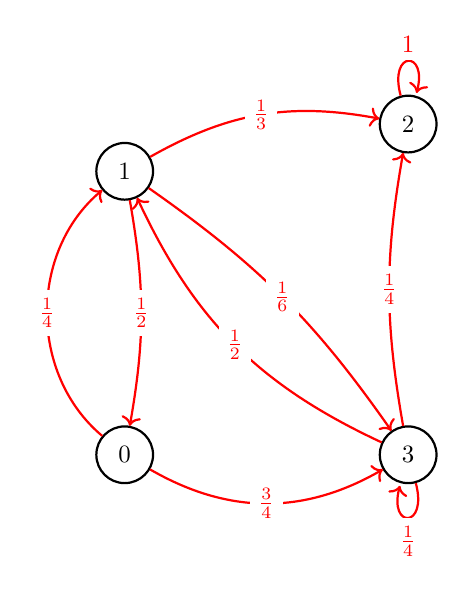
\begin{tikzpicture}[scale=1.2, every node/.style={scale=0.9}]
			% Nodes
			\node[circle, draw=black, thick, minimum size=0.8cm] (0) at (0,0) {0};
			\node[circle, draw=black, thick, minimum size=0.8cm] (1) at (0,3) {1};
			\node[circle, draw=black, thick, minimum size=0.8cm] (2) at (3,3.5) {2};
			\node[circle, draw=black, thick, minimum size=0.8cm] (3) at (3,0) {3};
			
			% Edges
			\path[->, red, thick] (0) edge[bend left=50] node[midway, fill=white] {\(\frac{1}{4}\)} (1);
			\path[->, red, thick] (0) edge[bend right=30] node[midway, fill=white] {\(\frac{3}{4}\)} (3);
			
			\path[->, red, thick] (1) edge[bend left=10] node[midway, fill=white] {\(\frac{1}{2}\)} (0);
			\path[->, red, thick] (1) edge[bend left=20] node[midway, fill=white] {\(\frac{1}{3}\)} (2);
			\path[->, red, thick] (1) edge[bend left=10] node[midway, fill=white] {\(\frac{1}{6}\)} (3);
			
			\path[->, red, thick] (2) edge[loop above] node[fill=white] {\(1\)} (2);
			
			\path[->, red, thick] (3) edge[bend left=20] node[midway, fill=white] {\(\frac{1}{2}\)} (1);
			\path[->, red, thick] (3) edge[bend left=10] node[midway, fill=white] {\(\frac{1}{4}\)} (2);
			\path[->, red, thick] (3) edge[loop below] node[fill=white] {\(\frac{1}{4}\)} (3);
		\end{tikzpicture}
	\end{center}
	
	\vspace{1em}
	
	\noindent This graph corresponds to the following one-step transition matrix:
	\[
	\vec{P} =
	\begin{bmatrix}
		0 & \frac{1}{4} & 0 & \frac{3}{4} \\
		\frac{1}{2} & 0 & \frac{1}{3} & \frac{1}{6} \\
		0 & 0 & 1 & 0 \\
		0 & \frac{1}{2} & \frac{1}{4} & \frac{1}{4}
	\end{bmatrix}
	\]
	
	\subsection{Classification of States}
	To analyze the \emph{long-term behavior} of a Markov chain, we must classify its states.
	
	\begin{definition}[Accessibility and Communicating Relation]
		For \(n \ge 0\), we say that state \(j\) is \textbf{accessible} from state \(i\) if and only if \(P_{i, j}^n > 0\). Moreover, it is trivially true that \(P_{i, i}^0 = 1\), which means every state is accessible from itself. Additionally, if two states \(i\) and \(j\) are accessible from each other (i.e., state \(j\) is accessible from state \(i\) and state \(i\) is accessible from state \(j\)), we say that they \textbf{communicate} and denote it as \(i \leftrightarrow j\).
		
		In the graph representation (see Definition~\ref{graph_markov_rep}), it is illustratively clear that \(i \leftrightarrow j\) if and only if there exist directed paths connecting \(i\) to \(j\) and vice versa. If two states communicate, they form an equivalence relation known as the \textbf{communicating relation}, which satisfies:
		\begin{enumerate}
			\item \textbf{Reflexivity}: for any state \(i\), \(i \leftrightarrow i\);
			\item \textbf{Symmetry}: if \(i \leftrightarrow j\), then \(j \leftrightarrow i\);
			\item \textbf{Transitivity}: if \(i \leftrightarrow j\) and \(j \leftrightarrow k\), then \(i \leftrightarrow k\).
		\end{enumerate}
		\label{accessibility_markov}
	\end{definition}
	
	Thus, the states of a Markov chain can be \emph{partitioned} into \textbf{communicating classes}—i.e., only members of the same class communicate with each other (courtesy of transitivity).
	
	\noindent For example, observe the following graph (assuming all weights \(P_{i, j} > 0\)):
	
	\vspace{1em}
	\begin{center}
		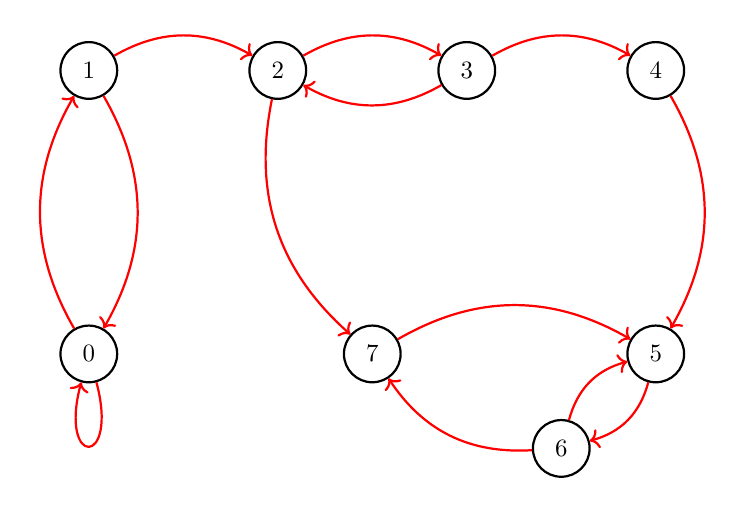
\begin{tikzpicture}[scale=1.2, every node/.style={scale=0.9}]
			% Nodes
			\node[circle, draw=black, thick, minimum size=0.8cm] (0) at (0,0) {0};
			\node[circle, draw=black, thick, minimum size=0.8cm] (1) at (0,3) {1};
			\node[circle, draw=black, thick, minimum size=0.8cm] (2) at (2,3) {2};
			\node[circle, draw=black, thick, minimum size=0.8cm] (3) at (4,3) {3};
			\node[circle, draw=black, thick, minimum size=0.8cm] (4) at (6,3) {4};
			\node[circle, draw=black, thick, minimum size=0.8cm] (5) at (6,0) {5};
			\node[circle, draw=black, thick, minimum size=0.8cm] (6) at (5,-1) {6};
			\node[circle, draw=black, thick, minimum size=0.8cm] (7) at (3,0) {7};
			
			% Edges
			\path[->, red, thick] (0) edge[bend left=30] (1);
			\path[->, red, thick] (0) edge[loop below, looseness=15] (0);
			\path[->, red, thick] (1) edge[bend left=30] (0);
			\path[->, red, thick] (1) edge[bend left=30] (2);
			\path[->, red, thick] (2) edge[bend left=30] (3);
			\path[->, red, thick] (2) edge[bend right=30] (7);
			\path[->, red, thick] (3) edge[bend left=30] (2);
			\path[->, red, thick] (3) edge[bend left=30] (4);
			\path[->, red, thick] (4) edge[bend left=30] (5);
			\path[->, red, thick] (5) edge[bend left=30] (6);
			\path[->, red, thick] (6) edge[bend left=30] (5);
			\path[->, red, thick] (6) edge[bend left=30] (7);
			\path[->, red, thick] (7) edge[bend left=30] (5);
		\end{tikzpicture}
	\end{center}
	
	We have the following communicating classes:
	\begin{itemize}
		\item \textbf{Class 1}: \(\{0, 1\}\)
		\item \textbf{Class 2}: \(\{2, 3\}\)
		\item \textbf{Class 3}: \(\{4\}\)
		\item \textbf{Class 4}: \(\{5, 6, 7\}\)
	\end{itemize}
	
	\begin{definition}[Irreducibility]
		A Markov chain is \textbf{irreducible} if all states belong to a single communicating class; that is, for every pair of states \((i, j)\), \(i \leftrightarrow j\).
		\label{irreducible_markov}
	\end{definition}
	
	\begin{lemma}
		A finite Markov chain (i.e., one with a finite number of states) is irreducible if and only if its graph representation is strongly connected; that is, every pair of vertices is reachable from each other.
	\end{lemma}
	\begin{proof}
		In the underlying digraph we draw an arc $i\to j$ iff $P_{ij}>0$.
		
		($\Rightarrow$)  \textit{Contrapositive.}
		Suppose the digraph is \textbf{not} strongly connected.  
		Then there exist vertices $i$ and $j$ with no directed path $i\to j$.  
		Hence $P^m_{ij}=0$ for every $m\ge 1$, so $i$ does not reach $j$ and the chain
		has more than one communicating class; it is therefore not irreducible.
		
		($\Leftarrow$)  Assume the digraph is strongly connected.  
		For any states $i,j$ there is a directed path
		$i=v_0\to v_1\to\cdots\to v_k=j$ with $P_{v_{\ell-1}v_\ell}>0$ for each $\ell$.
		Multiplying those positive probabilities gives
		\(
		P^k_{ij}=P_{v_0v_1}\cdots P_{v_{k-1}v_k}>0,
		\)
		so $i$ reaches $j$.  By symmetry, all states communicate; the chain is
		irreducible.
	\end{proof}
	
	\begin{definition}[Aperiodicity]
		For a discrete-time Markov chain with transition matrix \(\vec{P}\), define the
		\emph{period} of state \(i\) as
		\[
		\Delta(i)\;=\;\gcd\{\,m\ge 1 : P_{i,i}^{\,m}>0\}.
		\]
		The state \(i\) is \textbf{periodic} if \(\Delta(i)>1\) and
		\textbf{aperiodic} if \(\Delta(i)=1\).
		
		If a state is periodic, returns to \(i\) occur only at multiples of \(\Delta(i)\);
		equivalently, \(P_{i,i}^{\,m}=0\) whenever \(\Delta(i)\nmid m\).
		\label{aperiodic_markov}
	\end{definition}
	
	To determine if a Markov chain is aperiodic, we apply the following procedure, which can be carried out manually for simple graphs:
	\begin{enumerate}
		\item Partition the chain into its communicating classes.
		
		\item For each class, select an arbitrary state \(i\). Determine whether state \(i\) is aperiodic by identifying two or more return paths from \(i\) to itself in the graph representation. Let the lengths of these paths be \(\ell_1, \ell_2, \dots, \ell_m\) (this means that \(P_{i, i}^{\, \ell} > 0\)). Then state \(i\) is aperiodic if and only if
		\[
		\gcd(\ell_1, \ell_2, \dots, \ell_m) = 1.
		\]
		Ensure that the set \(\{\ell_1, \ell_2, \dots, \ell_m\}\) is exhaustive unless one of the values of \(\ell\) immediately yields \(1\) when computing the \(\gcd\).
		
		\item If a single state within a communicating class is found to be aperiodic, then all states in that class are aperiodic. Otherwise, the entire class is periodic, and the chain is not aperiodic.
		
		\item Repeat this check for all communicating classes to conclude whether the entire chain is aperiodic.
		
		\textit{Quick tip:} If the Markov chain is \emph{irreducible} and contains a self-loop (i.e., \(P_{i,i} > 0\)). Then we can immediately conclude the chain is aperiodic—a direct consequence of the procedure above.
	\end{enumerate}
	
	\noindent As a simple example:
	\vspace{1em}
	\begin{center}
		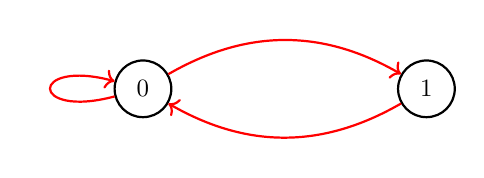
\begin{tikzpicture}[scale=1.2, every node/.style={scale=0.9}]
			% Nodes
			\node[circle, draw=black, thick, minimum size=0.8cm] (0) at (0,0) {0};
			\node[circle, draw=black, thick, minimum size=0.8cm] (1) at (3,0) {1};
			
			% Edges
			\path[->, red, thick] (0) edge[loop left, looseness=15] (0);
			\path[->, red, thick] (0) edge[bend left=30] (1);
			\path[->, red, thick] (1) edge[bend left=30] (0);
		\end{tikzpicture}
	\end{center}
	
	We can determine that the chain above is aperiodic because:
	\begin{enumerate}
		\item \(\Delta(0)\): \(\gcd(1, 2) = 1\), (Paths: \(0 \rightarrow 0\) and \(0 \rightarrow 1 \rightarrow 0\)).
		\item \(\Delta(1)\): \(\gcd(2, 3) = 1\), (Paths: \(1 \rightarrow 0 \rightarrow 1\) and \(1 \rightarrow 0 \rightarrow 0 \rightarrow 1\)).
	\end{enumerate}
	
	We continue with definitions and interesting results pertaining to stationary distributions.
	
	\begin{definition}[Recurrent States and Transient States]
		For $t\ge 1$, denote
		\[
		r_{i,j}^t
		\;=\;
		\Pr\!\bigl(X_t=j \text{ and } X_k\neq j \text{ for } 1\le k\le t-1 \mid X_0=i\bigr),
		\]
		i.e., the probability that the \emph{first} transition to state $j$ from state $i$ occurs at time $t$.
		We say the state $i$ is \textbf{recurrent} if $\sum_{t\ge 1} r_{i,i}^t = 1$; otherwise, if
		\[
		p \;:=\; \sum_{t\ge 1} r_{i,i}^t \;<\; 1,
		\]
		then $i$ is \textbf{transient}.  Thus, if $i$ is recurrent, with probability $1$ the chain returns to $i$ (in fact, infinitely often) when started at $i$; otherwise it returns only with probability $p<1$.
		In the transient case, the number of \emph{returns} to $i$ (after time $0$) is geometric random variable.
		
		Moreover, the \textbf{expected time} to first reach $j$ from $i$ (the hitting time) is
		\[
		h_{i,j} \;=\; \sum_{t\ge 1} t\, r_{i,j}^t .
		\]
		Note that if one state in a communicating class is recurrent, then all states in that class are recurrent; likewise for transience. Therefore, a Markov chain is recurrent if every state in the chain is recurrent.
		\label{recurr_states}
	\end{definition}
	
	\begin{definition}[Positive Recurrent State]
		If a state $i$ is recurrent and $h_{i,i}<\infty$, then $i$ is \textbf{positive recurrent}; otherwise (recurrent with $h_{i,i}=\infty$) it is \textbf{null recurrent}.
		\label{pos_recurr_states}
	\end{definition}
	
	\begin{definition}[Ergodic States]
		A state is \textbf{ergodic} if it is aperiodic and positive recurrent. Similarly, a Markov chain is ergodic if all of its states are ergodic.
		\label{ergodic_states}
	\end{definition}
	
	\begin{theorem}
		Any finite, irreducible, and ergodic Markov chain has a unique \textbf{stationary distribution} $\overline{\pi}$.
		Moreover, for each state $i$,
		\[
		\pi_i \;=\; \lim_{t\to\infty} P_{j,i}^{\,t} \;=\; \frac{1}{h_{i,i}},
		\]
		so $\pi_i$ is the limiting probability—independent of the initial state $j$—that the chain is in state $i$.
		It is as if the chain forgets its initial state far out in the future.
	\end{theorem}
	
	The proof of this remarkable theorem is out of scope for this note; however, one may enjoy this result with a concrete example.
	
	\noindent Consider the following.
	\vspace{1em}
	\begin{center}
		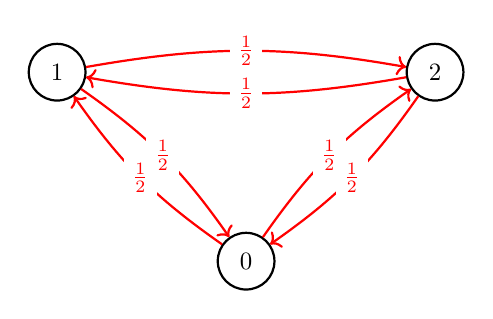
\begin{tikzpicture}[scale=1.2, every node/.style={scale=0.9}]
			% Nodes
			\node[circle, draw=black, thick, minimum size=0.8cm] (0) at (0,0) {0};
			\node[circle, draw=black, thick, minimum size=0.8cm] (1) at (-2,2) {1};
			\node[circle, draw=black, thick, minimum size=0.8cm] (2) at (2,2) {2};
			% Edges
			\path[->, red, thick] (0) edge[bend left=10] node[midway, fill=white]{\(\tfrac{1}{2}\)} (1);
			\path[->, red, thick] (1) edge[bend left=10] node[midway, fill=white]{\(\tfrac{1}{2}\)} (0);
			\path[->, red, thick] (0) edge[bend left=10] node[midway, fill=white]{\(\tfrac{1}{2}\)} (2);
			\path[->, red, thick] (2) edge[bend left=10] node[midway, fill=white]{\(\tfrac{1}{2}\)} (0);
			\path[->, red, thick] (1) edge[bend left=10] node[midway, fill=white]{\(\tfrac{1}{2}\)} (2);
			\path[->, red, thick] (2) edge[bend left=10] node[midway, fill=white]{\(\tfrac{1}{2}\)} (1);
		\end{tikzpicture}
	\end{center}
	
	One may easily verify that this chain is finite, irreducible, and ergodic.  
	The straightforward approach is to solve \(\overline{\pi}\vec{P}-\overline{\pi}=\vec{0}\) with the additional constraint \(\sum_i \pi_i=1\)—this method is of course general and applies to any Markov chain. Thus,
	\[
	\begin{bmatrix}
		\pi_0 & \pi_1 & \pi_2
	\end{bmatrix}
	\!
	\begin{bmatrix}
		0 & \tfrac{1}{2} & \tfrac{1}{2}\\[2pt]
		\tfrac{1}{2} & 0 & \tfrac{1}{2}\\[2pt]
		\tfrac{1}{2} & \tfrac{1}{2} & 0
	\end{bmatrix}
	-
	\begin{bmatrix}
		\pi_0 & \pi_1 & \pi_2
	\end{bmatrix}
	=
	\begin{bmatrix}
		0 & 0 & 0
	\end{bmatrix}.
	\]
	Therefore we obtain the system
	\[
	\begin{aligned}
		-\pi_0 + \tfrac{1}{2}\pi_1 + \tfrac{1}{2}\pi_2 &= 0,\\
		\tfrac{1}{2}\pi_0 - \pi_1 + \tfrac{1}{2}\pi_2 &= 0,\\
		\tfrac{1}{2}\pi_0 + \tfrac{1}{2}\pi_1 - \pi_2 &= 0,\\
		\pi_0 + \pi_1 + \pi_2 &= 1.
	\end{aligned}
	\]
	Solving yields \(\overline{\pi} = \bigl(\tfrac{1}{3},\,\tfrac{1}{3},\,\tfrac{1}{3}\bigr)\).
	
	Now we apply the theorem above to see if we obtain the same result. Immediately, by symmetry we deduce that \(\pi_0=\pi_1=\pi_2\), since the hitting time \(h_{i,i}\) is the same for every \(i\). Thus it suffices to compute \(h_{0,0}\). For convenience, let the random variable \(X_j\) denote the expected time to reach state \(0\) from state \(j\). Then we have the following recurrences (which can be solved as a linear system):
	\[
	\begin{aligned}
		X_0 &= \tfrac{1}{2}\bigl(1+X_1\bigr)+\tfrac{1}{2}\bigl(1+X_2\bigr),\\
		X_1 &= \tfrac{1}{2}\cdot 1 + \tfrac{1}{2}\bigl(1+X_2\bigr),\\
		X_2 &= \tfrac{1}{2}\cdot 1 + \tfrac{1}{2}\bigl(1+X_1\bigr).
	\end{aligned}
	\]
	Solving gives \(X_0=3\), hence \(\pi_0=\tfrac{1}{h_{0,0}}=\tfrac{1}{3}\), concluding our result spectacularly!
	
	In fact, the chain above is a special type of Markov chain known as a \emph{random walk}, which is often used to analyze algorithms.
	
	\begin{definition}[Random walk on undirected graphs]
		A random walk on an undirected graph \(G=(V,E)\) is a process in which a particle at vertex \(i\) moves at each step to a neighboring vertex along an incident edge, choosing each neighbor with probability \(1/\deg(i)\). Here \(\deg(i)\) denotes the degree of \(i\).
	\end{definition}
	
	\section{Counting}
	Many of the analyses shown here in discrete probability are riddled with \emph{counting}; for example, counting the number of successes to find the probability of success or counting the number of possible outcomes to establish a sample space (or a conditional sample space). In this segment, we aim to cover the mathematics of counting to make sense of many results shown definitively.
	
	\subsection{The Counting Principle}
	This is a mathematical shortcut to find the total number of possible outcomes from a series of collections. Suppose we have \(r\) collections, and each collection \(C_i\) has \(n_i\) elements. To find \emph{all} possible outcomes, we simply compute the \emph{Cartesian product} to obtain the \textbf{ordered} \(r\)-tuples. Thus,
	\[
	|C_1 \times \dots \times C_r| \;=\; \prod_{i=1}^{r} n_i,
	\]
	and the result tells us how many possible outcomes there are. We can see this fact is correct because in the first collection there are \(n_1\) elements to choose from, in the second \(n_2\) elements, and so on.
	
	For example, suppose Alice has three shirts, two pairs of pants, and three caps; the number of ways she can combine them is therefore \(3\times 2\times 3 = 18\) by the counting principle. Likewise, the number of legitimate telephone numbers of a \(9\)-digit sequence where the first digit must be \(1\) or \(9\) is \(2 \times 10 \times \dots \times 10 = 2\cdot 10^{8}\) by the counting principle.
	
	\subsection{\(k\)-Permutations}
	We are interested in choosing \(k\) elements from a collection of \(n\) \emph{distinct} elements (with \(k \le n\)) and then arranging them in a sequence—how many ways can we do this? By the counting principle, we have \(n\) choices for the first element, then \(n-1\) for the second, and so on, down to \(n-k+1\) for the \(k\)th element. (Note that we might select the same set of \(k\) elements more than once, but in different \textbf{orders}; this reflects the “arrangement’’ aspect of \(k\)-permutations.) Thus, the number of ways is
	\[
	n\,(n-1)\,\dots\,(n-k+1)=\frac{n!}{(n-k)!}.
	\]
	It is straightforward to verify that this equality holds. In particular, the number of ways to arrange all \(n\) distinct objects—the case of \(n\)-permutations—is obtained by setting \(k=n\) in the formula above, yielding \(n!\).
	
	\subsection{Combinations}
	We are again interested in choosing \(k\) elements from a collection of \(n\) \emph{distinct} elements (\(k\le n\)), \textbf{but} now the order (i.e., arrangement) in which they are chosen does not matter. First note that there are \(k!\) ways to order any fixed set of \(k\) selected elements; accordingly, the number of \(k\)-permutations equals \(k!\) times the number of \(k\)-combinations. Hence the number of combinations is
	\[
	\frac{n!}{k!\,(n-k)!}=\binom{n}{k}.
	\]
	This fact underlies the \emph{binomial distribution}: when counting the number of successes in \(n\) Bernoulli trials, we need \(\binom{n}{k}\) because we do not care about the order in which the \(k\) successes occur, which greatly simplifies the computation.
	
	\subsection{Partitions}
	Suppose we have a collection of \(n\) \emph{distinct} elements. We wish to \emph{partition} them into \(r\) groups: the first group having \(n_1\) elements, the second \(n_2\) elements, and so on, with \(\sum_{i=1}^{r} n_i = n\). Because the order in which the elements are chosen does not matter in each group, we obtain, by repeated use of combinations and the counting principle, that the number of ways to form a partition of type \((n_1,n_2,\dots,n_r)\) is
	\[
	\binom{n}{n_1}\,
	\binom{\,n-n_1\,}{n_2}\,
	\binom{\,n-n_1-n_2\,}{n_3}\,\dots\,
	\binom{\,n-n_1-\dots - n_{r-1}\,}{n_r}.
	\]
	Writing each binomial in factorial form,
	\[
	\frac{n!}{n_1!(n-n_1)!}\;
	\frac{(n-n_1)!}{n_2!(n-n_1-n_2)!}
	\,\dots\,
	\frac{(n-n_1-\dots-n_{r-1})!}{n_r!\,(n-n_1-\dots-n_{r-1}-n_r)!},
	\]
	and canceling the telescoping terms (with \((n-n_1-\dots-n_r)! = 0! = 1\)) yields
	\[
	\frac{n!}{n_1!\,n_2!\,\dots\,n_r!}
	= \binom{n}{n_1;n_2;\dots;n_r}.
	\]
	
	\medskip
	\noindent\emph{Example.}  
	To find the number of anagrams of the word \texttt{COLOSSAL}, note that there are eight \emph{unique} positions which can be partitioned into five groups according to repeated letters: \(G_C=1\), \(G_O=2\), \(G_L=2\), \(G_S=2\), and \(G_A=1\). Hence the number of anagrams is
	\[
	\frac{8!}{1!\,2!\,2!\,2!\,1!}=5040.
	\]
	
	\section*{Acknowledgement}
	I would like to acknowledge \emph{Probability and Computing: Randomization and Probabilistic Techniques in Algorithms and Data Analysis}, 2nd edition, by Michael Mitzenmacher and Eli Upfal, as the primary source of reference for these notes.
	
\end{document}
